%% University of Lincoln Computer Science Thesis Template

%% @version     1.0.4
%% @lastchanged 12th June 2020

% The document class -- remove [harvard] if you want
% numeric-style referencing.
\documentclass[harvard,bibliography=totoc]{lincolncsthesis}

% Custom packages that you need to include
% Packages you intend to use
% ..

% For example, if you want to render 
% the document in a different font you can
% use something like: 

% \usepackage{gentium}

\usepackage{url}
\usepackage{rotating}
\usepackage{ftnxtra}
\usepackage{fnpos}
\usepackage{listings}
\usepackage[definitionLists,hashEnumerators,hybrid]{markdown}

%\usepackage[hybrid]{markdown}
%\usepackage{lscape}


\definecolor{codegreen}{rgb}{0,0.6,0}
\definecolor{codegray}{rgb}{0.5,0.5,0.5}
\definecolor{codepurple}{rgb}{0.58,0,0.82}
\definecolor{backcolour}{rgb}{0.95,0.95,0.92}

\lstdefinestyle{codestyle}{
    backgroundcolor=\color{backcolour},   
    commentstyle=\color{codegreen},
    keywordstyle=\color{magenta},
    numberstyle=\tiny\color{codegray},
    stringstyle=\color{codepurple},
    basicstyle=\ttfamily\footnotesize,
    breakatwhitespace=false,         
    breaklines=true,                 
    captionpos=b,                    
    keepspaces=true,                 
    numbers=left,                    
    numbersep=5pt,                  
    showspaces=false,                
    showstringspaces=false,
    showtabs=false,                  
    tabsize=2
}

\lstdefinestyle{codestyle}{
    backgroundcolor=\color{backcolour},   
    commentstyle=\color{codegreen},
    keywordstyle=\color{magenta},
    numberstyle=\tiny\color{codegray},
    stringstyle=\color{codepurple},
    basicstyle=\ttfamily\footnotesize,
    breakatwhitespace=false,         
    breaklines=true,                 
    captionpos=b,                    
    keepspaces=true,                 
    numbers=left,                    
    numbersep=5pt,                  
    showspaces=false,                
    showstringspaces=false,
    showtabs=false,                  
    tabsize=2
}
\lstset{style=codestyle}


% Somewhere to put commands in shorthand form
\newcommand{\footcaption}[1]{\caption[#1]{#1\footnotemark}}
\newcommand{\mono}[1]{\texttt{#1}}
\newcommand{\tableref}[1]{Table \ref{#1}}
\newcommand{\figureref}[1]{Figure \ref{#1}}
\newcommand{\footref}[1]{Footnote \ref{#1}}
\newcommand{\sectionref}[1]{Section \ref{#1}}
\newcommand{\eqnref}[1]{Equation \ref{#1}}


% Comments in the report for identifying key points/questions
\newcommand{\noteGeneral}[1]{\textit{\color{cyan}#1}}
\newcommand{\noteCF}[1]{\textit{\color{red}#1}}
\newcommand{\noteComment}[1]{\textit{\color{green}#1}}
\newcommand{\noteAttention}[1]{\textit{\color{blue}#1}}
\newcommand{\source}[0]{\textbf{\textit{\color{magenta}This claim needs a source.}}}
\newcommand{\wording}[0]{\textbf{\textit{\color{magenta}This statement is unclear and needs re-wording.}}}


% Listings (Code segments)
\renewcommand{\lstlistingname}{Code Segment}
\renewcommand{\lstlistlistingname}{List of \lstlistingname s}
\newcommand{\coderef}[1]{Code Segment \ref{#1}}

% figure
\newcommand{\picturesque}[3]{\begin{figure}\centering\includegraphics[width=0.8\textwidth]{#1}\caption{#2}\label{#3}\end{figure}}

\newcommand{\noteAndrew}[1]{\textbf{\color{amber}#1}}


% Your thesis details -- edit the file at the path below
% so it shows your name, title, etc. 
% Put the correct details in here
\author{Jack Stevenson}
\thesisDegree{Master of Science Intelligent Vision}
\thesisSubmissionDate{August 2020}

% If your thesis title spans over three lines, prepend the command with \Large!
\title{\bfseries Optimisation of a hippocampus model with test-driven GPU parallel programming}

% Supervisor details
\thesisSupervisor{Dr. Charles Fox}

% Set up the bib files which are gonna be used
% throughout this document
% Add in the .bib files you wish to add 
% into your document here. If you want to
% include others, just copy this line and
% change the path!

\addbibresource{bib/miscellaneous.bib}
\addbibresource{bib/software.bib}
\addbibresource{bib/model.bib}


\begin{document}

% start of document
% --------------------------

% Make the title. You can pass an option to this
% to render the title differently, like so:
%\maketitle[logo-first]
\maketitle


% The abstract of the thesis
\begin{abstract}

%\textbf{\color{red}Hippocampus is great! It is the stuff that dreams are made on.\newline
%GPU programming is great! It's like all the crap that deep learning people go on about but with actual real programming and architecture.\newline
%Let's do both great things at once!}
The Hippocampus is a useful biological model of spatial memory.
Functioning models of hippocampus may be useful for robot navigation.
Previous work, \citep{foxandprescott2010A,foxandprescott2010B, saul2011} developed a computer model to mimic the hippocampus, implemented in serial code.
However, serial execution is very slow at scale.
This means that the model only functioned in very small `toy' environments.
Modern GPUs can massively parallelize execution of neural networks. 
This is usually done for the backpropagation of multilayer perceptrons, but they similarly offer the possibility of speeding up more realistic biological networks such a this hippocampus model.
This project aims to modify the model's existing serial learning process to be more parallel, using GPU hardware.
Our research finds that the model may be suited to using the CPU for small environments, however in simulated larger environments that the model may need to learn would greatly benefit from parallel execution.

\end{abstract}

\begin{acknowledgements}
%Firstly, I want to thank somebody, and somebody else.\footnote{Here is a footnote} Here is another thing.
% Fox, C for helping to steer me away from my percieved biases and supporting me.
% Hi Charles,

% This will be paragraph will be removed for the final submission, however I thought that I should let you know that most of this report has been written as "I am the expert".
% Because of this I feel it is possible to miss underpinning the argument with proper academic literature.
% If there is a claim in the Literature Review/Methodology/Project Requirements(Aims, Tools and toolsets, project management, etc.) please let me know by placing \mono{\\source} at the end of the relevant sentence.
% Likewise, if a sentence does not make sense, then please can you place \mono{\\wording} in the relevant sentence. 
% I have split sentences into individual lines to make this process easier.

% I have also included points where I am not sure on the correct approach to it, and have indicated these points in different colours.
% \begin{itemize}
%     \item \noteCF{Red}: Questions
%     \item \noteComment{Green}: Wording problems
%     \item \noteAttention{Blue}: extra information which might not be needed.
% \end{itemize}

% Thank you in advance,
% Jack.

I would like to thank my supervisor, Charles Fox for helping to steer me away from my perceived biases and pushing me to not just settle on adequate results.


\end{acknowledgements}

% Print out the table of tables and table of figures and
% tell the template we're about to start the body of the
% thesis.

\thesisTables
\thesisBodyStart


% start of thesis body
% ---------------------------

% Include introduction
\chapter{Introduction}

%\textbf{\color{red}CF: start with the big picture: ie hippocampus is important and could be used by %robots. BUT the current implementation is too slow for robots to use!   THEREFORE we are going to %fix it!}
%\textbf{\color{red}CF: gradually work down to the specific task}
%\textbf{\color{red}CF: parallel computing provides a possible solution …  Parallel computing is %great !  because …. (keep brief, this is not the lit review)}
%\textbf{\color{red}CF: A particular model of HC is ...}
%\textbf{\color{red}CF: BUT it is really hard to make sure the implementation still works in the %same way …}
%\textbf{\color{red}CF: REFACTORING is great and will resolve the second big but because ….}
%\textbf{\color{red}CF: one para, clearly state what this thesis is going to deliver (and why.)}

The hippocampus is an important area of the brain involved in spatial memory. 
This allows us to consider it as a method of robot navigation. 
This can be done by mapping the specialised cells in the hippocampus to activations in a machine learning system.
However this approach can be considered slow due to the serial learning process, and is unsuitable for real-time use.
Despite this, there are sections of the model which would benefit from parallelisation, making a real-time system using this approach more viable.

One model of the hippocampus is the unitary coherent particle filter, as proposed by \cite{foxandprescott2010A}. 
This model utilises the wake-sleep algorithm proposed by \cite{hintonDBN2006}.
This is useful as it allows for the model to respond to immediate changes to inputs. %{\color{green} needs verifying by reading papers.}
The model architecture %{\color{green} and data flow}
is explored in more detail in \sectionref{subsubsec:ucpf} .

We can use modern compute technology, such as GPUs to parallelise the learning process of the model. 
By parallelising our code, we enable the easy horizontal scaling of the model by reducing the workload on a given processing unit. 
As part of this process, we will need to re-implement the code to allow for a parallel implementation of the serial learning process.

A process for re-implementing code is refactoring.
This involves re-writing code without changing the external behaviour of the code.
This is beneficial to our project as it provides us a methodology to maintain behaviour when as we switch the model to use a parallel implementation.

In this thesis, we will refactor the Hippocampal model of \cite{saul2011} into a new parallel TensorFlow based implementation.
We do this by wrapping the functions in unit tests, which will enable us to make the model run faster and be used on robots in real time.
% using \noteCF{Fowler’s theory of refactoring\wording} wrapped by unit tests, to make the model run faster and able to be used on real time robots.
% reconsider 

% The Introduction feels like I might need a bit more, but not sure what to talk about, maybe criticisms of refactoring or the model, but that feels like it should be in literature review.

%There are multiple types of refactoring as it covers a variety of changes, such as renaming variables to have more meaningful names, reorganising functions to be in a more appropriate place and vectorisation of loops.
% Include this as footnote at end of the above line?
% More examples of changes that can be considered refactoring can be found here:
% https://refactoring.com/catalog/index.html
%

% Related work 
\chapter{Background and Related Work}
\section{Review of Hippocampus models}
\subsection{Hippocampus biology}
The hippocampus \cite{andersen2006hippocampus}  is involved in the creation and consolidation of memories, in a circuit along with the Entorhinal Cortex (EC) and Dentate Gyrus (DG).
The main function of the hippocampus is thought to be the consolidation of associative memories and spatial memory.
As such it can be considered suitable for navigation within an environment, associating each place with sensory memories about that place.

The hippocampus is comprised of four main sub-fields: CA1, CA2, CA3 and CA4.
However, the classical view of the hippocampal circuit only considers the CA1 and CA3 sub-fields, along with the EC and DG.
The circuit accepts input from external sources and the response from the CA1 sub-field.
This is then passed to the DG which sparsifies the EC output.
The output of the EC is also passed to the CA3 sub-field along with the output of the DG.
The CA3 sub-field also accepts recurrent connections.
This allows it to consolidate interactions between old
 and new stimuli.
CA3 then projects its output to the CA1 sub-field, which provides the main output to the rest of the limbic system.
This structure is shown in \figureref{fig:hippocampus}

\picturesque{figures/lit_biology/CajalHippocampus.png}{Visual representation of the hippocampal circuit, modified from the \cite{imghippooriginal} original by \cite{imghippo}.}{fig:hippocampus}

% \begin{figure}
%     \centering
%     \includegraphics{}
%     \caption{Classical Circuit of the hippocampus}
%     \label{fig:bio_hippocampus}
% \end{figure}
%\textbf{\color{red}CF: you can mostly paraphrase this from my previous papers here. It is traditional to include some pictures of brains here. HC is supposed to look like a seahorse and there are pictures of that.}
\subsection{Hippocampal model - Unitary Coherent Particle Filter}
\label{subsubsec:ucpf}
%\textbf{\color{red}CF: you can mostly paraphrase this from my previous papers here. You can include figures showing the model structures here.}

% CF: the reader will not understand the model. You need to show a diagram of the model itself and describe its components with full mathmatical details.
The initial model of the unitary coherent particle filter of hippocampus (UCPF-HC) by \cite{foxandprescott2010A} uses handset weights to initialise the model and understand how it initially evolves. 
This is further expanded to use sensors to differentiate between locations within a simple environment.

 \picturesque{figures/lit_biology/alan_model.png}{Illustration of the hippocampus model showing data flows and hippocampus regions. SURF features are the new visual inputs. (Subiculum circuit not shown.) from \cite{saul2011}}{fig:ourcircuit}

The model is comprised of 4 main areas, an EC representation, a DG representation, the CA3 subfield and the CA1 subfield.
The EC and DG are used to provide input from the outside world to the model, encoding them into lamellae.
They project to the CA3 sub-field, which is represented in the model by a modified Temporal Restricted Boltzmann Machine(TRBM), proposed by \citep{hintonDBN2006}.
This allows the CA3 sub-field to be represented by the joint probability distribution:
\begin{equation}
    P(x_t, x_{t-1}, z_t) = \frac{1}{Z}\exp\sum_t(-x_t' W_{x_t'x_t'} x'_{t-1} - x'_tW_{x'_tz'_t}z'_t )
\end{equation}

In this distribution, $z$ represents a boolean observation vector, $x$ represents a boolean hidden state vector and the weight matrices between them.
This distribution, in conjunction with the modification of the standard Temporal Restricted Boltzmann Machine allows for a deterministic update, obtaining maximum \textit{a posteriori} estimates,

\begin{equation}
    \hat{x_t} \leftarrow arg \max   P(x_t|\hat{x_{t-1}},z_t) = \{\hat{x_t}(i)=(P(x_t(i)|\hat{x_{t-1}},z_t) > \frac{1}{2})\}_i
    \label{eqn:post}
\end{equation}

%  this does not make sense
% \wording
which is considered to be a zero temperature limit of the annealed sequential Gibbs sampler.
This sampler gives a set of boolean values, which can then be used to identify where the model believes it is in the environment. 
These boolean values can then be decoded into the CA1 sub-field, which projects back to the EC, completing the circuit.




% \note{paragraph on how different parts of the model map to the Hippocampus}
% \begin{figure}
%     \centering
%     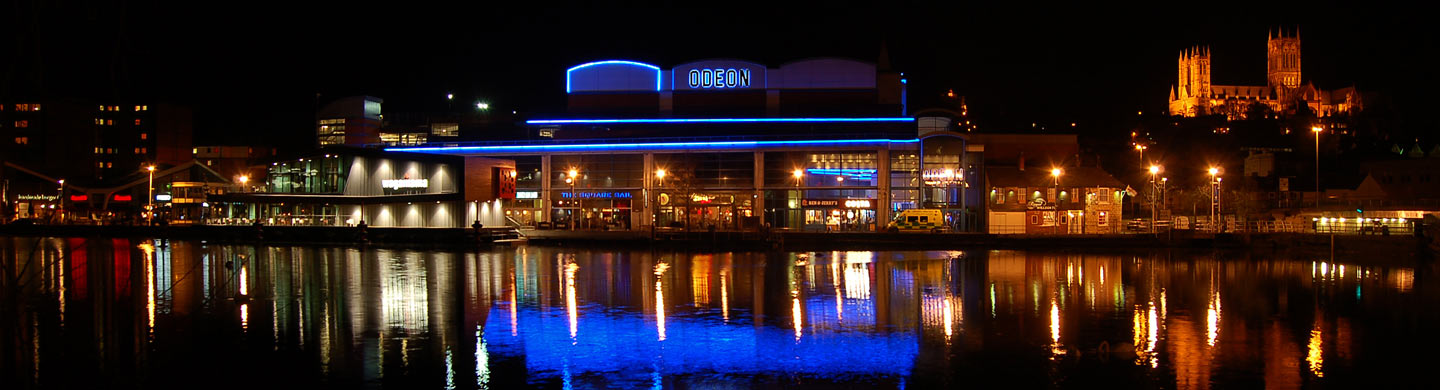
\includegraphics{figures/brayford.jpg}
%     \caption{Map of hippocampus to model.}
%     \label{fig:}
% \end{figure}
\section{Parallel Computing Technologies}

% CF: you need to introduce this section, why is it here, what will it be doing?
% We have so far reviewed hippocampus biology and models.
% The aim of this study is to make those models go faster in computational implmentations.
% Paralization is a way to make them go faster.
% There are many forms of a prallelisation technology.
% We will need to choose one.
% So this section will review these options and make this choice.
We have currently reviewed the biology of the hippocampus and a model that uses it.
This model currently uses a serial process to learn.
The aim of the study is to make the model learn faster in computational implementations.
One method of making them go faster is parallelisation.
However there are many forms of parallelisation technology.
As such we will need to choose one, focusing on GPUs only.
So this section will review these options and make a choice on the technology to use.

\subsection{Low level}
\subsubsection{CUDA}
CUDA is a proprietary parallel framework for interfacing with NVidia GPUs.
It is a C-based programming language, and uses kernel functions to run code in parallel.
CUDA handles the launching of kernels and memory management through the use of the CUDA runtime\citep{nvidiacuda}.
The CUDA runtime makes the assumption that memory on the host (CPU/RAM) and memory on the device (GPU) are separate.
This means that data needs to be transferred between the CPU and GPU when the GPU is needed.
This creates overhead from the copy operations, as well as spawning the CUDA runtime process.
On the other hand, this approach to the initialisation of CUDA means that GPU is only in use when needed, and can be considered free when not in use, allowing multiple programs access to the same hardware. %\textit{{\color{blue}Need to verify this claim. Was written in "I am the expert mode"}}

\subsubsection{OpenCL}
OpenCL is an open-source parallel framework for interfacing with GPUs. 
As an open framework, it is capable of working on both NVidia GPUs and AMD GPUs.
However there are only a few functions in the standard.
This means that external libraries, such as clBLAS \citep{clblas} or CLBlast \citep{clblast} are needed to aid machine learning applications.

\begin{minipage}{\linewidth}
\begin{lstlisting}[caption=Psuedocode of CL Initialisation and Kernel Execution, label=code:cl_init]
//Initialise OpenCL, run once
context -> CL_Context
queue -> CL_Command_Queue(context)
kernel_source -> CL_Program_Source(readfile(kernels))
program -> CL_Program.of(kernel_source)
program.build()

//Run a kernel
inputA -> vector<int>[N]
inputB -> vector<int>[N]
output -> vector<int>[N]
bufferA -> CL_Buffer.ofSize(length(inputA)*sizeof(int))
bufferB -> CL_Buffer.ofSize(length(inputB)*sizeof(int))
bufferC -> CL_Buffer.ofSize(length(output)*sizeof(int))
queue.writeVectorToBuffer(inputA, bufferA)
queue.writeVectorToBuffer(inputB, bufferB)
kernel -> CL_Kernel(program, KERNEL_FUNCTION_NAME)
setKernelArgument(kernel, bufferA)
setKernelArgument(kernel, bufferB)
setKernelArgument(kernel, bufferC)
queue.runKernel(kernel)
queue.readBufferToVector(bufferC, output)

return output

\end{lstlisting}
\end{minipage}


When programming for pure OpenCL, a developer is often writing the code that directly interfaces with the GPU.
The libraries reduce the amount of code that needs writing by providing optimised routines, however these routines often perform a single function.
Thus they are not suitable for neural network calculations as each operation would need to be transferred between the CPU and GPU, increasing overhead.

% In contrast, CUDA has these libraries built into the API.\wording  
% Furthermore, CL code directly interfaces with the GPU.
% This makes CL extremely low level.
% As such it is not as suitable for machine learning using biology based computation.



In addition, the OpenCL runtime requires a large amount of setup code to begin working with it.
The setup code is trivial to create, as seen in \coderef{code:cl_init}.
However it adds a large amount of preparation code for each call to a parallel kernel.
This increases the amount of code for a given function, which is likely to increase overall running time, and reduce the readability of the function.



As OpenCL is able to run on multiple brands of GPUs, there are many different implementations of the standard.
However, as CUDA is directly tied to NVidia GPUs, there is only a small distinction between the CUDA API and CUDA Runtime, as it is closely tied to NVidia GPUs.
There have been attempts to integrate the CUDA API onto other devices, using
OpenCL as the base for it's processing.
We discuss a couple of these implementations below.

% \noteCF{CF: Unlike CL, these is less disticntion between API and implmention in CUDA, because it's so tied to NVida cards.  In theory, there is a CUDA API and one or more implemnetations, which could include one or more architectures able to implement it.   Just recently for example there have been attempts to implement the CUDA API by compilint it into CL then using any CL backend, such as FPGA etc as well as GPU.}

% This means that some common parallel operations, such as matrix multiplication would need to be self implemented.
% This reduces the available time for testing the model.

% \noteCF{CF: really? aren't there available BLAS or Eigen implenetations for OpenCL , or other matrix libs? the real reason to not use CL is that it is oo low level, TF is a beter match for nueural level stuff due to its graph structure.}

% Because of the self implementation, it is likely that the functions needed for machine learning applications would be not properly optimised.
% This makes it less likely that the system will be able to operate as fast as possible.
% On the other hand, more proprietary frameworks, such as CUDA, already have highly optimised functions for common machine learning applications.
% This makes OpenCL an unsuitable parallel library for our project.
% \begin{itemize}
%     \item Bloat of CL code.
%     \item Should probably have a code example here to help explain the bloat
%     \begin{itemize}
%         \item lot of initial setup
%         \item large amount of memory usage
%     \end{itemize}
%     \item Good point: Gives a lot of control to the user
%     \item Obfuscation/abstraction of strings
% \end{itemize}



% Open standard, thus anyone can use it. Moderately clunky to use. When using it developers are often working directly with what gets executed, rather than working with highly optimised and tested library functions. This can be useful in some cases, however most applications do not need this level of control/responsibility.

% \subsubsection{OpenMPI}
% Old standard
 
% originally developed in 1991

% Parallelisation is obtained by passing messages between devices.

% This makes it suitable for distributed applications.
% This might be useful in the future, however our project only uses a single machine.

% Should we consider OpenMPI? It's parallelisation via messages similar to network packets, which makes better for distributed workload, but as our workload focuses on single machine workload, it adds to much overhead.

\subsubsection{ROCm/HIP}
ROCm is a low level parallelisation framework for AMD Hardware, developed by AMD.
It uses a single source model.
This allows it to work on different hardware platforms, such as CPUs, APUs and GPUs.

It has different variations depending on the target platform and applications, such as servers (ROCk) and machine learning (mlOpen).
This allows it to be similar to CUDA.
It also supports HIP code, which allows ROCm programs to run on CUDA-enabled GPUs.

However, it is a relatively new technology, in comparison to CUDA and OpenCL \cite{rocminsights}.
This means that it does not have the same amount of support as CUDA for machine learning.
This makes it unsuitable for our project, as it can require a large amount of setup compared to using native CUDA hardware.
% Very similar to CUDA

% Allows CUDA based software to run on Non-nvidia GPUs

% Developed by AMD

% reference point https://moorinsightsstrategy.com/wp-content/uploads/2016/11/AMDs-ROCm-Software-Helps-Accelerate-HPC-and-Deep-Learning-by-Moor-Insights-and-Strategy.pdf

\subsubsection{SYCL}
In contrast to OpenCL and CUDA, SYCL is a relatively new low level platform for parallel computing.
It builds upon the OpenCL standard, however unlike OpenCL it incorporates high level routines as well.
As such, it sits between the code and other low-level architectures such as OpenCL, CUDA and OpenMP.

SYCL programmes use a single source paradigm.
This allows for parallel kernels to be included as part of the original source.
This reduces the overhead for loading the kernels into the program, unlike OpenCL.  
It also means that code written for SYCL can be compiled for different platforms, such as CUDA and HIP/ROCm. 
By allowing the compiler to handle how the code is compiled and initialised, it can be assumed that the routines used are heavily optimised for the architecture.

%Summary for SYCL
Like ROCm, SYCL is relatively new.
As such, there is not as much support for SYCL implementations of higher level libraries.
There has been an attempt to port Tensorflow, which originally uses a CUDA backend, to a SYCL b backend (find sycl tensorflow), however it is in the alpha stages, thus it may not be stable enough for our purposes.  

% Relatively new ~5 years old

% Inspired by OpenCL

% Has multiple "flavours"
%     - different versions of the same source for different compilers/apis
%     - e.g. Clang, Compute for CUDA, OpenMPI, hip/ROCm

% Single source multiple compiler
%     - Can be compiled for different frameworks
%     - Kernels are written in source of code files, don't need to be loaded as external file/string

% Let compiler handle initialisation of parallel framework

% structure:
%     code -> SYCL -> Backend(Cuda/OpenCL/OpenMPi)

% not all backends provide pre-built kernels

% {\color{green}
% Point of interest: levels of data parallelism
% \begin{itemize}
% \item Basic data, i.e. no syncronisation needed. e.g. add 2 vectors
% \item Work-group, i.e. reduction style kernels
% \item Heirachical, i.e. element-wise parallel operations in work-groups
% \end{itemize}
% }

% reference point https://www.khronos.org/registry/SYCL/specs/

% sycl-2020-provisional.pdf


\subsection{High level parallel libraries for Python}
\label{subsec:highlevellibs}
There are different parallel libraries for high level languages which can be used to bind native language code, such as Java and Python, to the low level libraries like CUDA and OpenCL. 
As the computational implementation of the UCPF model by \cite{saul2011} uses Python, we consider a subset of Python bindings as there are many different bindings in various stages of implementation compliance.

% We focus on a subset of Python bindings to the low level libraries described above as the model by \cite{saul2011} uses python.\wording
% We consider a subset of python bindings as there are many different implementations of the low level libraries in various stages of implementation compliance.\wording

\subsubsection{PyOpenCL}
PyOpenCL\cite{kloeckner_pycuda_2012} is a binding to the OpenCL library.
Kernels are written as strings, and the PyOpenCL library compiles them into executable code.
This provides the benefit of being able to easily write and understand the kernels.
However, software written with OpenCL requires a lot of setup in order to execute it, as seen in \coderef{code:cl_init}.

PyOpenCl only provides bindings to the OpenCL API, thus external libraries such as clBLAS would need to be imported as well to make use of them, which can be considered a non-trivial task.
In addition, many machine learning backends, e.g. Keras and Theano, focus more on CUDA based implementations, as opposed to an OpenCL implementation.
Implementing functions of the UCPF-HC model as OpenCL kernels would optimise the model, however it would also increase the overall complexity of the software, an outcome that refactoring aims to avoid.
This makes PyOpenCL unsuitable for our project.


% As PyOpenCL only provides the bindings to the OpenCL library, common machine learning operations, such as matrix multiplication, would need a kernel written specifically for it.
% This detracts from the development of the unit tests for the model, and reduces overall time spent on identifying slow areas of code.
% In addition, OpenCL is a standard and has little support for machine learning.\wording
% This is due to many machine learning backends, such as Keras and Theano focusing more on the CUDA API.
% The lack of support for machine learning further suggests that OpenCL will become more unsuitable for complex tasks, and only used for teaching an understanding of parallel computing.\wording


\subsubsection{CuPy}

CuPy is an array manipulation library accelerated by CUDA. 
It aims to be a NumPy compatible library~\citep{cupy_learningsys2017}. 
This means it provides functions that operate the same as NumPy functions.
This is useful as it would make the transition from NumPy, which is a serial array manipulation library that the model currently uses, to a parallel system easier.

However part of our development process is to create a system that is easy to update in the future.
Whilst CuPy could be used as a parallelisation framework, it's similarity to the current serial implementation, NumPy, does not push the boundary far enough to allow for different frameworks to be experimented with. 
Furthermore, CuPy does not integrate with machine learning backends, such as Keras.
This is detrimental because it does not allow for future builds of the backends, which include Restricted Boltzmann Machines and other machine learning architectures aside from neural networks to be easily integrated with out existing model, provided the implementations are able to pass the tests.
In addition, CuPy does not scale across multiple GPU devices, which indicates that versions of the model with several thousands of neurons would be incompatible with using CuPy as the backend for handling the learning.


\subsubsection{Theano}

Historically, the first widely used data flow graph system was Theano. 
Theano evolved over several years and eventually influenced newer libraries such as TensorFlow and Torch.
Both of these libraries have replaced Theano but they still owe many architectural and implementation features to it.

Theano works by defining mathematical operations and data points as nodes on a directed acyclic graph \citep{theano}. 
This graph is then compiled to a highly optimised form.
By compiling the graph, it allows for reduced memory consumption, and the transfer of the model to a hardware accelerated device, such as GPUs.
GPU computation is done on CUDA enabled devices.

This parallel computation makes Theano suitable for vector and matrix calculations, which allows it to be useful for neural network calculations.
This makes Theano suitable for our purposes as our model heavily uses
matrix calculations as part of it's calculations.

However, Theano is an older library, with support from the official maintainers, MILA stopped as of 2017 \citep{milaTheano2017}. 
This means that it is less likely to support current hardware, and will not support future hardware.
As such, we will not be using Theano for this project as our intent is to allow for future parallelisation of the model.




\subsubsection{PyTorch}
PyTorch is a set of Python bindings to the Torch Machine Learning Tensor library, developed by Facebook.
As a tensor library, it has mathematical functions implemented, as well as machine learning algorithms.
It is primarily developed for batch processing, using custom cache allocations to reduce synchronisation barriers and maximise device usage.

A large proportion of the PyTorch machine learning functionality is provided by the libTorch library.
This allows for efficient operations as libTorch is written in C/C++.
This does cause some overhead compared to working in pure Python, however the highly optimised C code negates the overhead.
In addition the Python language does have the ability to compile it's code as C code.
This makes the overall processing much faster, and more suitable for deployment purposes.

The authors of PyTorch focus on the philosophy of `everything is a program' \cite{paszke2019pytorch}.
This suggests that software written for PyTorch can be considered as a collection of small, independent programs.
By decoupling implementation from usage, the philosophy makes it suitable for unit testing as each program can be tested independently.
In addition, testing can be performed on the integration of these programs.

Applying the philosophy of PyTorch to our system, we have three major programs: the creation of the environment, the learning process and the verification process, which would simplify our system for future work, as it can be targeted for a particular subsystem, with full integration being tested near the end of the process.
However, implementing the model in this manner greatly increases the scope of our refactoring, and does not benefit our optimisation focus.

\subsubsection{Tensorflow}

Like Theano, Tensorflow is a tensor based machine learning library that is being developed by Google.
It originally used a graph-based execution model, with tensor operations being defined as nodes on the graph.
However as of Tensorflow 2 it uses an eager execution model.
This makes it useful for prototyping, however eager execution also reduces the overall optimisation of the model as it is interpreting the human-readable code as opposed to the machine readable binary.
\begin{minipage}{\linewidth}
\begin{lstlisting}[caption=Tensorflow Code Example, label=code:tensorflow1, language=python]
input_1 = tf.Variable(shape=(5,1))
input_2 = tf.Variable(shape=(1,3))
operation_matmul = tf.matmul(input_1, input_2)
operation_sum = tf.reduce_sum(operation_matmul)

\end{lstlisting}
\end{minipage}

As Tensorflow 2 is a machine learning library, it primarily works with the Keras backend.
This is because Keras is a simple to use framework for learning deep netwroks.
Due to the versitility of deep learning in performing different tasks, such as Writing Music \citep{dhariwal2020jukebox}, Voice Puppetry \citep{deepneuralvoicepuppetry} or Medical Analysis \citep{coviddeepprognosticdiagnostic}, it makes deep models extremely useful outside of research based tasks.
In contrast to deep learning, our model is considered shallow.
This means that we will not be working with Keras or deep learning in our study, however having them as an option for future work is beneficial.
This is because the developers of these libraries may implement functions for Restricted Boltzmann Machine Learning in the future, and these will likely be highly optimised by being low level functions with high level invokers.

Despite the focus on Deep learning and neural networks with Keras~\citep{tensorflowtutorials}, Tensorflow can also be used as a maths library.
This is useful for our purposes as it can act as a replacement for NumPy, without being extremely similar. 
It also allows the model to operate on a different maths framework which should enable easier porting of the network to different frameworks/libraries.

%\textbf{\color{red}CF: you might want to review some parallel profiler tool here as well?   because we are now finding that it might be useful.  what does actually mean to profile a parallel program?  wall clock time vs compute time.  might be useful to find any problems with the latest version -- i am surprised that its not faster yet.}

\subsubsection{Choice of framework}
A study by \citep{bahrampour2015comparative} compares different machine learning frameworks.
The study looks at five frameworks, Caffe, Neon, Theano, Torch and Tensorflow.
Their results indicate that in terms of speed, Theano and Torch are the best options, for small and large networks respectively.
However this study was published in 2016, which means that the results may not reflect current standards in these libraries, such as Theano discontinuing development and the release of Tensorflow 2.0.

The study also indicates that Tensorflow is shown to have the most flexibility. 
This flexibility makes it simpler to create software with it as it allows for variances when refactoring the model.
It should also be noted that GPU tests in the study use Tensorflow with cuDNN v2, whereas the other listed libraries use cuDNN v3.
This was because these were the officially supported versions, thus optimisations in cuDNN versions may have affected the results.

Another reason for choosing Tensorflow over other machine learning libraries 
is that it allows for low level data flow graphs to be generated, whereas many other machine learning libraries for Python focus on Multi-layer Perceptron model architectures. It is more beneficial to have control over the data flow graphs for this model as we are using modified versions of the standard Temporal Restricted Boltzmann Machine equations. 


% \noteCF{CF: its not clear here that the reason reason is that most of the others only do MLPs. Tensorflow is lower level letting you mke your own dataflow graphs lik you need here.}   

% Study by \note{https://arxiv.org/pdf/1511.06435.pdf}
% Their results show that Theano and torch are the best options for speed, THeano for small and Torch for large.
% However Tensorflow is the most flexible.
% Tensorflow is also middle of the road?
% Make more sense to use Torch/Theano, Tensorflow flexibility allows for more creative solutions to be available.

% Rework this paragraph
% Although Tensorflow is primarily developed for the CUDA platform, there are also custom tensorflow build targeting the SYCL platform.
% This allows us to exercise the power of Tensorflow on non-CUDA enabled GPUs, which is useful for further work where the model is transferred from a simulation setting to a real world example.
% However for simplicity's sake we will be using stock Tensorflow.
% This will allow for simple verification of our work by other researchers.\noteAttention{This is probably weak/unnecessary. Should probably try to consider better reason.} 
\section{Software Engineering and refactoring}

\section{Profiling Results}
% Should include figures for initial implementation and the final implementation(Test id 15)
\subsection{Number of calls}
From \figureref{fig:ncc} we can see that the most called function, a lambda in the SURFExtractor module is part of the setup process, meaning the relevant functions are \mono{boltzmannProbs} in the rbm module, the \mono{fuse} function from the cffun module and the \mono{err} function in the learn weights module.


\begin{figure}
    \centering
    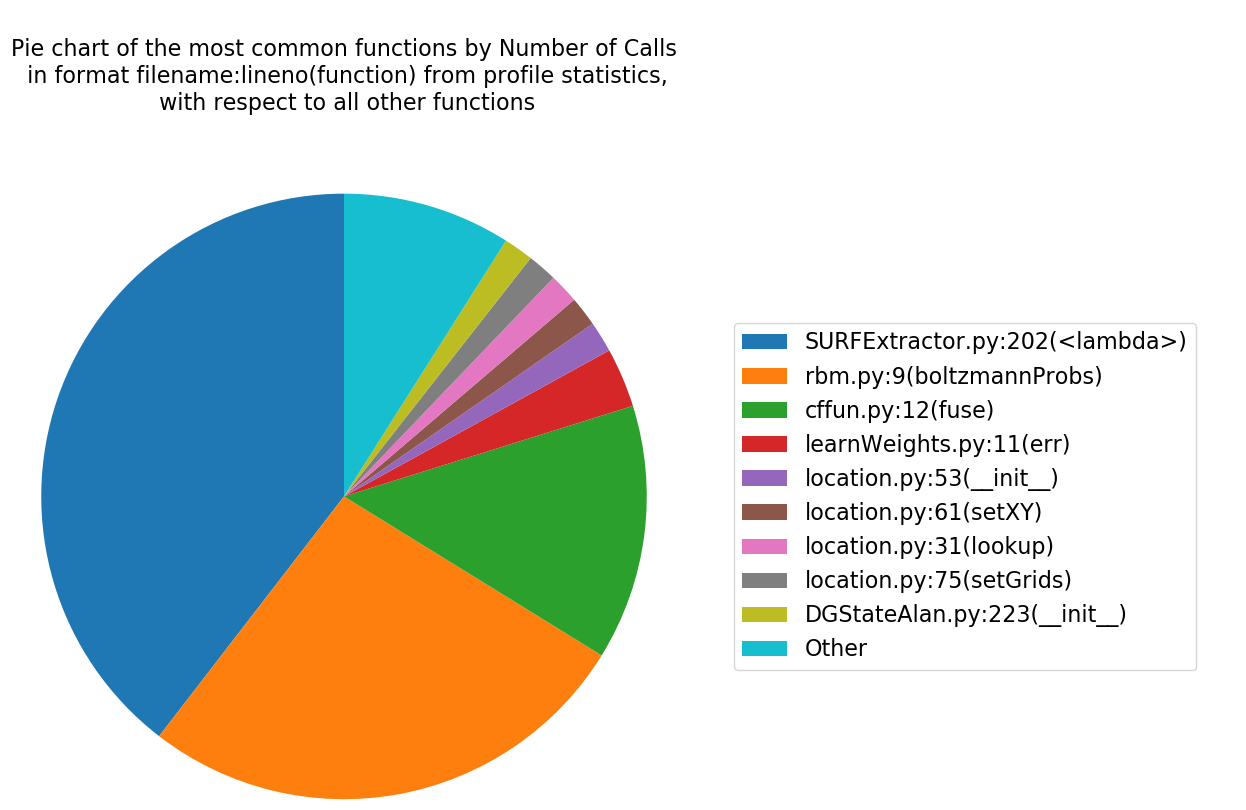
\includegraphics[width=0.7\textwidth]{figures/res_profiling/number_calls_cpu_crop.png}
    \caption{Number of calls for the CPU implementation of the model.}
    \label{fig:ncc}
\end{figure}

\begin{figure}
    \centering
    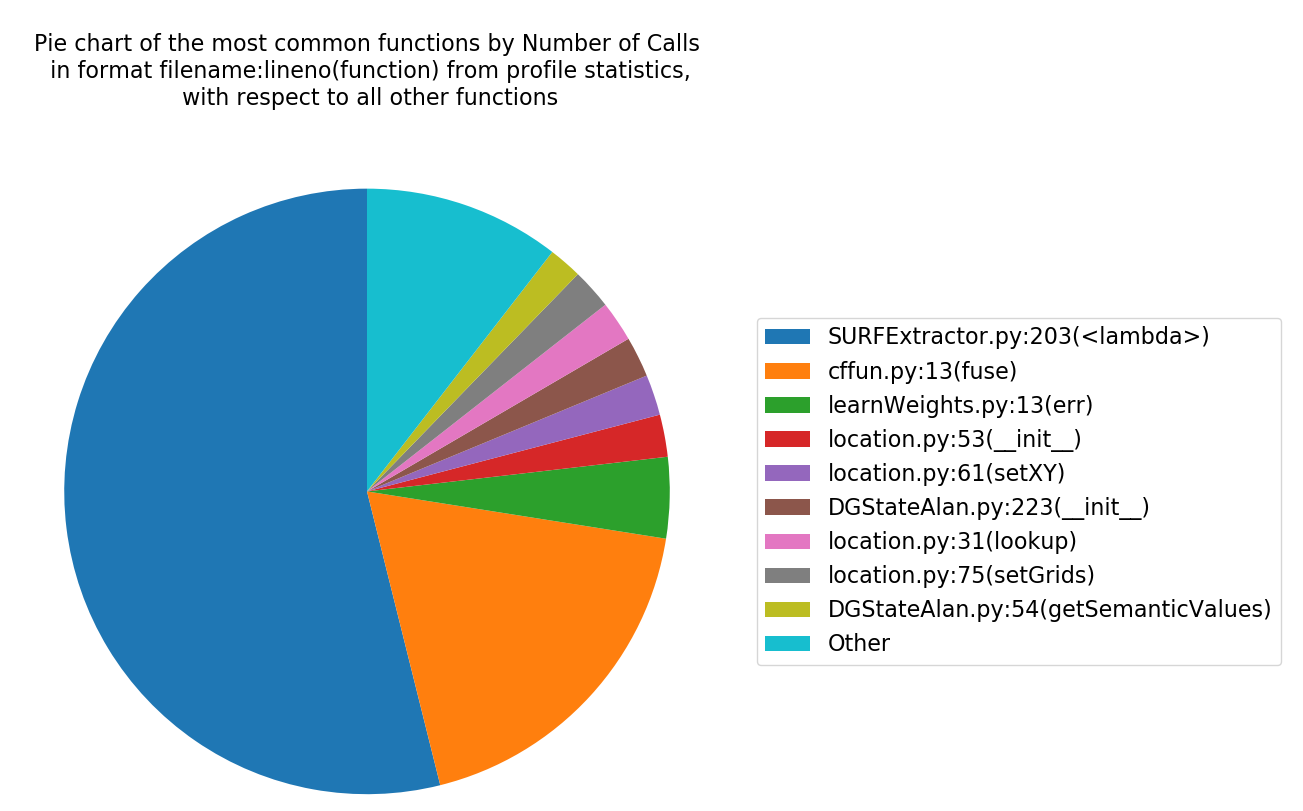
\includegraphics[width=0.7\textwidth]{figures/res_profiling/number_calls_gpu_crop.png}
    \caption{Number of calls for the GPU implementation of the model.}
    \label{fig:ncg}
\end{figure}

In contrast, profiling the Tensorflow version (\figureref{fig:ncg}) shows the lambda function from SURFExtractor taking a larger proportion of the total number of calls.
This is likely due to the usage of the \mono{tf.function} decorator optimisation.
The decorator converts the function into an optimised Tensorflow data call graph, which is loaded into the memory of the GPU at runtime.



Tensorflow processes the calls to the function such that the profiler only records the first time each call to \mono{boltzmannProbs} is hit, as opposed to everytime.
The \mono{cffun\#fuse} function has approximately the same amount of calls, and can probably be reduced by applying the \mono{tf.function} decorator.
Finally the \mono{learnWeights\#err} function has a constant number of calls across both implementations as it is not affected by the randomness of the model.


\subsection{Total time}

The more interesting profiling results come from the total time spent executing the function, excluding calls to other functions.
Initially the main functions that take the most time are the \mono{learn} function of the \mono{learnWeights} module, the \mono{boltzmannProbs} function of the \mono{rbm} module and the \mono{fuse} function of \mono{cffun} module as seen in \figureref{fig:ttc}.

After applying the parallel refactoring, the \mono{learnWeights\#learn} function takes a larger proportion of the overall time taken, as seen in \figureref{fig:ttg}.
The \mono{cffun\#fuse} function also has an increase in the proportion of time taken.
However, given that the overall time taken increases with a small amount of nodes, it indicates that there may be an underlying algorithmic problem which causes this behaviour.

\picturesque{figures/res_profiling/tot_time_cpu_crop.png}{Total time for function calls for the CPU implementation of the model.}{fig:ttc}

\picturesque{figures/res_profiling/tot_time_gpu_crop.png}{Total time for function calls for the GPU implementation of the model.}{fig:ttg}


In addition, the \mono{boltzmannProbs} function appears to have a large reduction in time taken.
However this is likely due to the \mono{tf.function} decorator function mapping the original function to a data call graph that runs purely on the GPU, which the Python profiler does not have access to.
This can be seen when using the line profiler on the \mono{boltzmannProbs} function.

%insert listing or similar thing depicting the output of line profiler, with full excerpt in an appendix.
\coderef{profiling:line_boltzmann} shows the results of profiling the \mono{boltzmannProbs} function line by line. 
It can be seen that the main bottleneck is the multiplication of the inputs and weights, taking approximately 60\% of the overall time.
This is likely due to the asynchronous nature of matrix multiplication, which is applied across a given dimension of the inputs. 


\begin{minipage}{\linewidth}
\begin{lstlisting}[caption=Line by line profiling of the rbm\#boltzmannProbs function in eager execution mode, label=profiling:line_boltzmann]
Total time: 237.186 s
Function: boltzmannProbs at line 9

Line #      Hits         Time  Per Hit   % Time  Line Contents
==============================================================
     9                                           @profile
    10                                           #@tf.function
    11                                           def boltzmannProbs(W, x, axis=0):      # RETURNS THE PROBABILITY OF A NODE BEING ON
    12    252240  143312866.0    568.2     60.4      mult = tf.tensordot(W, x, axis)
    13    252240   12193753.0     48.3      5.1      squeezed = tf.squeeze(mult)
    14    252240    6917896.0     27.4      2.9      E_on  = -squeezed       #penalty is the negative of the reward (just to make it look like energy
    15    252240   20604441.0     81.7      8.7      E_off = 0.0*E_on
    16    252240   13057317.0     51.8      5.5      Q_on = tf.math.exp(-E_on)       #as energy is negated, we have e^(reward)
    17    252240   12601996.0     50.0      5.3      Q_off = tf.math.exp(-E_off)
    18    252240   28258157.0    112.0     11.9      P_on = Q_on / (Q_on + Q_off)
    19    252240     239234.0      0.9      0.1      return P_on
\end{lstlisting}
\end{minipage}





\subsection{Unit tests}
\label{subsec:unittest}
{
A big problem with creating and improving software is that it is likely to break.
This is especially true when refactoring to speed up the code.
This is due to changes in underlying implementation creating side effects in the code.
These side effects cause the code to break, and if left unchecked increases the technical debt, which accrues as a natural part of the software development life-cycle.

\begin{minipage}{\linewidth}
\begin{lstlisting}[caption=Example unit to be tested, label=code:unit, language=python]
def boltzmannProbs(W, x, axis=0):
    """
    :param W: Input Weight Matrix
    :param x: Input Vector Matrix
    :param axis: Axis of contraction
    :return: activation probabilities
    """
    reward = tf.tensordot(W, x, axis)
    E_on  = tf.negative(reward)
    E_off = 0.0*E_on
    Q_on = tf.math.exp(-E_on)
    Q_off = tf.math.exp(-E_off)
    P_on = tf.math.divide(Q_on, tf.math.add(Q_on, Q_off))
    return P_on
\end{lstlisting}
\end{minipage}

Unit tests are a method of both reducing technical debt and ensuring that behaviour remains the same.
This is because the tests are used to verify behaviour after refactoring a unit.
A unit can be considered any functional object, however we define a unit as a custom function in the code.
An example of a unit can be seen in \coderef{code:unit}.
}



{
A test is a wrapper function that provides known inputs to the unit and checks the output of the unit against a known output.
The check is done via an assert statement.
An assert statement fails if the values that the assertion is checking do not match.
We define a test function as a singular concept on the unit being tested.
This allows us to understand the nature of the unit for that concept.
It also reduces confusion on what a given test is meant to do.
This reduces technical debt as future developers are not having to figure out what the 
purpose of a given test is, which increases productivity.
An example of a test can be seen in \coderef{code:test}
}



\begin{minipage}{\linewidth}
\begin{lstlisting}[caption=Example test for a unit, label=code:test, language=python]
def test_rbm_small():
    input_weights = np.array([[.1, .2], [.3, .4]])
    input_vector = np.array([.5, .6])
    calculated_results = rbm.boltzmannProbs(input_weights, input_vector)
    actual_results = np.array([0.54239794, 0.5962827])
    assert_almost_equal(calculated_results, actual_results,
                            err_msg="[BoltzmannProbs] Calculated results are not equal to actual results to 7 decimal places.")
\end{lstlisting}
\end{minipage}

{
%A big problem with the improvement of software is that it breaks when you change it. You are trying to speed it up but u change its functionality.   [introduce a problem]
%[sets you up to describe a solution]
%Units tests are an amazing way to fix this problem.  
%what is a unit test? 
%    what is a unit?
%        a function?  a class?  a file ?
%    what is a test?
%        one call of a unit? many calls of a unit?
%            many calls with a similar theme?
%        Used for testing how functions handle inputs and whether actual behaviour is what we expect.
%                using assertions
%                    say what is an assertion
%        show code examples  
%    martin fowler defined unit test as ...
 
 }      


\subsubsection{Test Driven Development and HC-UCPF}
Test Driven Development is a method of developing software that focuses on writing tests before writing code.
This allows the developer to write valid code the first time round, and does not need to spend long hours debugging the code.
This works well for new projects.
However our project involves refactoring an existing project.
Thus we can not follow test driven development to the letter.
But we can use the approach of test driven development as part of the refactoring process.
This means we write our tests and ensure that the existing code passes them.
This also has the benefit of helping to understand the purpose of the code.

By refactoring code in this manner, it helps with the process of debugging.
This is due to being able to pass the system inputs to the tests, and seeing what is causing the error.
Furthermore, from our definition of the unit test, we can obtain a hierarchical approach to debugging.
This is due to each of our functions being units, and invoking other functional units within our system.

For example, the function \verb|learn| in learnWeights.py\footnote{Found at \url{https://github.com/A-Yakkus/hclearn/blob/msc2020/learnWeights.py\#L16}} invokes the \verb|boltzmannProbs| function in rbm.py\footnote{Found at \url{https://github.com/A-Yakkus/hclearn/blob/msc2020/rbm.py\#L9}}.
If an error occurs during the learn function with respect to the \mono{boltzmannProbs} function, we can pause execution of the learn function and run the current inputs through our tests to find where the erroneous behaviour occurs.
Once we understand the erroneous behaviour, it can be considered trivial to fix it.
This would then allow successive invocations of the system to run without encountering the error. 

    % (though disputed by other people x y and z in these ways..)
    % what they do:
    %     they assure us that each unit works
    %     that allows us to try changing a unit
    %             eg to optimise
    %     it also allows delta debugging:
    %         hierarchy of unit tests
    %         find a bug by looking at red/green and homeing in
    %     what this is great
    %         saving tons of time! instant bug detection and localistion
    % TDD: write tests first
    % Refactoring: fowler's approach: how to optimise other peoples code  (vs TDDm is different)
    %     % Our case has it different as we already have functions implemented.
    % Parallel debugging:
    %   parallel is especially important use case here
    %         [NB we already told the reader about parallel techs, so we can refer to that now]
    %   new big idea here -- using fowler refactors to make parallel debugging tolerable !  is  big deal.



\subsection{Refactoring with Unit Tests}

Unit tests are traditionally used for the creation of software, as they are designed to help a developer create software.
This is because you can define the expected behaviour of a function and work to that definition.
However they can also be used in conjunction with profiling for speeding up known functions via refactoring.
This is because we can write the tests for a function that is causing the bottleneck from profiling.
We can then develop a new version of the function with Tensorflow, using these tests to preserve behaviour.

% As mentioned above, technical debt is created as part of the software development life-cycle.
% Technical debt is where software uses a quick lazy approach to code creation over properly developed code.
% In test driven development, technical debt occurs from developing the software without using tests.
% Refactoring can be used to reduce the technical debt created by developing a project.
% As an existing project, the HC-UCPF has technical debt.
% This indicates that refactoring will help reduce the overall technical debt.

% What is technical debt? 
% How is it created?

% What is refactoring?
% Why does it solve technical debt?

% Who is Fowler?
% What are his ideas?
% Why are they a good approach to refactoring?


A prominent figure in the field of refactoring is Martin Fowler.
Fowler describes unit testing as being situational, with a unit referring to an agreed upon identifier, such as a function, class or object, and a test referring to a fast, low-level implementation of the unit, focusing on a small part of the system ~\citep{fowlerUnit2014}.

Fowler suggests a hat-based approach to refactoring.
This means that as a developer, you would wear different metaphorical hats depending on the job.
Whilst wearing a particular hat, you purely focus on that job.
This reduces the chance of getting confused on what you are doing when working on the code.

% How does this relate to our project?
% \begin{itemize}
%     \item create unit tests to help understand what is going on with the code
%     \item implement new version for chosen parallel lib
%     \item integrate into system
%     \item full details in section 3.1
% \end{itemize}
% Fowler's Keynote speeches are the star here, namely the hat system. Our hats are testing (for unit tests), creation (for new tf code), integration (for implementing functions into system), ?system analysis (for delving into the namespace at specific points in execution/call stack and understanding what is going on)?

For our project, we are refactoring the model to allow for parallel execution of the learning process via unit testing.
This will also have the effect of making the learning easier to understand moving forward.
Hence we are reducing the technical debt of the project.
This allows us to create a number of hats for the different tasks, as follows:
\begin{itemize}
    \item A hat for the creation of unit tests.
    \item A hat for the development of parallel functions using Tensorflow.
    \item A hat for managing the integration of the parallel functions into the overall system.
\end{itemize}
% \noteAttention{What do these hats do?}
These hats can help guide the development of the project.
By developing the project in this way, we can control the scope of the refactoring, and keep it focused on the learning process, rather than the setup or evaluation.

Using the unit tests as a base for our refactoring is useful as it allows for faster system analysis in the event of a crash.
This is because the stack trace displayed when a crash occurs usually identifies the line that caused the crash.
This relies on the developer understanding the system to know how to fix it.

However our hierarchical approach to creating the unit tests reduces the amount of knowledge required.
This is because the inputs can be retrieved from a breakpoint in the debugging process, and then transferred to being inputs to a test script.
This test script then runs the unit tests on all functions and nested functions within that get invoked from the crash causing line.
Thus the overall time needed to fix the crash gets reduced as the unit tests identify how the crash is caused, making it easier to fix.
Furthermore, by reducing the amount of knowledge needed to understand the system at the onset of a project in this manner, we are able to curb the growth of future technical debt that the system may obtain.
% Why is this approach good for this method?
% \begin{itemize}
%     \item Allows for faster system analysis/debugging
%     \begin{itemize}
%         \item when code errors we get stack trace
%         \item stack trace usually identifies where problem is.
%         \item having unit tests for the identified problem makes it easier to identify problem and fix
%     \end{itemize}
%     \item reduces future technical debt
%     \begin{itemize}
%         \item functions often grow in scope
%         \item this allows for a trigger for when function is doing too much
%         \item KISS principle
%     \end{itemize}
% \end{itemize}



% We have only considered serial programming for refactoring
% however we are moving to a parallel approach
% this makes the software run asynchronously
% which makes it harder to identify where a problem lies

% This can be solved using unit tests in the fowler approach
% we can use the tests with inputs being the workgroups of the kernel launches
% This allows us to identify which workgroup is causing the problem.
% By identifying the problem input, we can work backwards through the software to find the first mutation which leads to the error.





% % Method
% \chapter{Methodology}
% 
CF: I sugget restructure:
GENERAL METHODS
   describing the general processes you will be using
EXPERIMENTS
   subsection for each specific refactoring you will do, corresponding to each result






\section{Other optimisations}
% \noteCF{ consider having a new section/theme on memory optimisation. so far we only thought about speed optimisation. but you are hitting on memory limits now.  use the same unit test methods to make sure optimisations are working.}
\subsubsection{Memory optimisation via data types}
As well as optimisations for speed, we can also optimise for memory.
This is useful because larger networks require more memory to train.
However memory is a finite resource.
When Tensorflow converts from numpy floating point array and python floats to being 64 bit float tensor.
This is not suitable for GPU processing.
This is because GPU's have the best efficiency when working on 32 bit floats.
This optimisation was found after inflating the size of the CA3 to see how it affected the time of the learning process after optimisation.
Furthermore there is a reduction in precision of the model, however the effect of this is can be considered negligible on overall performance of the model. 






CF: i suggest don't confuse methods with results here.  Introducing the error function optimisation is a method. The finding that it takes 20pc times is a result. it should go in the result along with the other informtion you mention here.







% \begin{markdown}

% Profiling the parallel version 
% #. shows a lot of conversions of numpy arrays and python ints/floats to tensorflow tensors
% #. this is due to it being done "on the fly"
% #. however this can be reduced, as tensorflow slicing and numpy slicing is the same
% #. thus move the conversions outside for loops defining time/epochs
% #. Speed up occurs (approx, 14\% at 1000 nodes) \note{i.e. PROFIT!}


% Rabbit Hole
% #. Scanning codebase for slower functions
% #. see `sum` keyword in error function
% #. use timeit to time how long it takes to run 10000 invocations consecutively for sizes [10, 100, 1000, 10000]
% #. results for it are [8s, 80s, 800s, 8700s]
% #. seems like good candidate for our optimisation process
% #. do optimisation process (unittests etc)
% #. get results of [1e-2s, 1e-1s, 1s, 10s]
% #. optimised version shows speed up, integrate into system
% #. run check to see whether speed up helps
% #. it doesn't (800s over 440s)
% #. bad optimisation. Good thing we can revert to pre-optimisation thanks to version control

% tf.function


% \end{markdown}

% % Method
% \chapter{Results}
% \section{Unit Test Results}
% Probably should email Charles about whether to include unit test results as part of the results section, or as part of appendix/poster.
    %CF: yes would be good to show some red and green here
%            (actually just green!)
% E.g. Unit tests -> Function integration results -> Size results -> Profiling results
% on poster have initial tests and and refactored tests.


% Figure using numpy, figure using tensorflow
After writing the unit tests we can use tools to automatically run them.
This allows us to monitor and manage the unit tests.

\picturesque{figures/res_unit_tests/numpy.png}{Unit test results for the NumPy version on CPU of the \mono{boltzmannProbs} function.}{fig:unit_numpy}

The initial tests were written with respect to the existing code, and to show a variety of behaviour for the function.
As such the tests will always pass, as seen by the green ticks in \figureref{fig:unit_numpy}
The tests showing as skipped (grey circle with line through it) are tests that are expected to fail.
This helps to manage the behaviour of the model.

\picturesque{figures/res_unit_tests/tensorflow.png}{Unit test results for the Tensorflow version on GPU of the \mono{boltzmannProbs} function.}{fig:unit_tensorflow}

As each test focuses on a single aspect, we can compare between the different versions of the model.
For example, the first test executed is the test on an array of large complex numbers.
This case is unlikely to occur, as it is not normally encountered in regular use.
On the GPU, this test takes approximately 1000ms, as seen in \figureref{fig:unit_tensorflow}.
In contrast, the test only takes 50ms on the CPU, seen in \figureref{fig:unit_numpy}.
This is a 20x slowdown in the GPU version, which is likely due to the effect of initialising Tensorflow.
Subsequent tests then show similar times to the NumPy versions, with several tests on the GPU matching or improving upon the NumPy equivalent times.

The test that shows the most interesting behaviour is the 1000 by 1000 test, which seems to indicate that the GPU version is slower by approximately 50\%. 
This is likely an anomalous result, as the GPU version matches the CPU version on most of the other    tests.
% The most interesting test is the 1000 by 1000 test, which seems to indicate that Tensorflow is slower on larger matrices.\wording
% This is unlikely however, and likely hardware dependent.

\pagebreak
\section{Function Timing}
\begin{table}[ht]
    \centering
    \resizebox{\linewidth}{!}{
        \begin{tabular}{|c|c|c|c|c|c|}
            \hline
            TEST ID & PARALLEL FUNCTION IMPLEMENTATION DETAILS & SIZE(of CA3) & TIME(s) & MAZE & TRAIN TYPE \\ \hline
            0 & Initial Implementation & 86 & 83.323  & PLUS & FULL \\ \hline
            1 & boltzmannprobs & 86 & 407.743 & PLUS & FULL \\ \hline
            2 & boltzmannprobs and addBias & 86 & 410.667 & PLUS & FULL \\ \hline
            3 & boltzmannprobs, addBias and hardThresh & 86 & 408.420 & PLUS & FULL \\ \hline
            4 & addBias and hardThresh & 86 & 89.255  & PLUS & FULL \\ \hline
            5 & addBias & 86 & 90.315  & PLUS & FULL \\ \hline
            6 & hardThresh & 86 & 85.431  & PLUS & FULL \\ \hline
            7 & trainPriorBias and hardThresh & 86 & 85.334  & PLUS & FULL       \\ \hline
            8 & trainPriorBias, invsig and hardThresh & 86 & 85.753 & PLUS & FULL \\ \hline
            9 & invsig and hardThresh & 86 & 84.903 & PLUS & FULL \\ \hline
            10 & invsig & 86 & 86.566  & PLUS & FULL \\ \hline
            11 & trainPriorBias and invsig & 86 & 86.791 & PLUS & FULL \\ \hline
            12 & trainPriorBias & 86 & 86.705 & PLUS & FULL \\ \hline
            13 & outer convienience function & 86 & 284.001 & PLUS & FULL \\ \hline
            14 & outer and boltzmannProbs & 86 & 428.402 & PLUS & FULL \\ \hline
            15 & outer, boltzmannProbs and Tensorflow random & 86 & 423.419 & PLUS & FULL \\ \hline
            16 & outer, highly optimised boltzmannProbs and Tensorflow random & 86 & 352.254 & PLUS & FULL \\ \hline
            17 & outer, decorated, highly optimised boltzmannProbs and Tensorflow random & 86 & 335.582 & PLUS & FULL \\ \hline
        \end{tabular}
    }
    \caption{
        Table of results comparing different functions as we parallelise the learning process.\footnotemark
    }
    \label{tab:results_table_functions}
\end{table}
\footnotetext{
    Results were gathered on a AMD FX8320 CPU (3.5GHz clock speed), 16GB 1600MHz Quad channel RAM and ASUS GT710-SL-2GD5 GPU (Uses Nvidia Geforce GT710 technology)
    \label{foot:system}
}
\tableref{tab:results_table_functions} shows how parallelising a given set of functions affects the runtime of the system after integration. 
The test id column refers to which test is being run.
The second column is defining which functions have been parallelised, with test 0, being CPU only functions.
The size column refers to the size of the CA3 sub-field, which is kept at 86 to help maintain consistency across different implementations.
The time column is the average wall clock time it takes to run the system. 
An average time is used to account for differences at the operating system level, such as interrupts and transfer overhead, which can occur at different times.
The final two columns give insight into the environment the model is learning (see \figureref{fig:plus_maze}, and the different methods of training the model.
These training methods include using the DG only, using handset weights only or using random weights only.
We opted to use all three training types to show that our optimisations can apply to each method.

It can be seen that there are two distinct bands of time, depending on the parallel functions integrated.
This is likely due to the number of calls to the \mono{boltzmannProbs} and outer functions, which results in multiple data transfers that is expensive.

Test IDs 16 and 17 show a further optimised version of the \mono{boltzmannProbs} function.
This is because the initial optimised \mono{boltzmannProbs} function was a translation of the original \mono{boltzmannProbs} function.
However Tensorflow does not have a replacement for the NumPy dot function.
This means that the multiplication of a matrix and scalar value does not work in Tensorflow.
To get around this limitation, an if statement for type checking was used.
But this added several unnecessary operations to the code.
Thus a more optimised form of the function, which primarily depends on the \mono{tf.tensordot} function is used, with inputs being forced into matrices before being passed to the function.
The decorator applied to the \mono{boltzmannProbs} function in test ID 17 is \mono{tf.function}. This provided the optimisation of compiling the function into a data flow graph instead of executable Python code.   
This resulted in the model being faster, and the version used for further analysis.


\chapter{Methods, Experiments and results}
As we are using test driven development in conjunction with profiling to guide the refactoring, we present our general methodology for refactoring and then each optimisation technique.
Alongside each optimisation, we provide results and analysis on what each optimisation does to the model.
Finally, we analyse the profiling and verify the model after all optimisations.

\subsubsection{Understanding the model for refactoring}

% \noteCF{CF: I think all of this should go in Methods chapter, it is real work. You need to show off a lot more of the actyal work you have done refactoing into TF. eg. giv many code examples of before and after functions.}

Before we can perform good refactoring of the model, we first need to understand how the model works, and what can be done to limit the variation in overall results that are seen.
We discuss how the computational implementation of the model works, and how randomness can affect results, alongside minimising the effects of randomness. 

The Unitary Coherent Particle filter of Hippocampus (UCPF-HC) model was initially developed in 2010, when serial computing was prevalent.
The learning method, contrastive divergence \citep{hintonDBN2006} is a primarily serial processing method, with each successive sample requiring the previous one.
This means that there are limited points of parallelisation in the learning process.

There are two key operations in our implementation of the learning process that should be parallelised, the calculation of individual probabilities for each input type to the model (biases, recurrent values, odometry and sensors) and the fusion of these probabilities into a singular joint probability table.
These operations can be considered parallel as each node of the model is independent of the others for these operations, meaning that a parallel worker can be applied to each node for the calculation, which should reduce the overall time to learn.


\subsubsection{Randomness in the UCPF-HC}
The UCPF-HC model uses randomness in two points of the execution of the system, in building the representation of the world and determining which neurons are active in the hidden state of the Temporal Restricted Boltzmann Machine (TRBM).

Pseudo random number generators (pRNGs) are used to create the random numbers for the model's learning process.
However many pRNGs generate random numbers using a serial algorithm.
% \wording
This is a problem in parallel computing as each calculation thread operates independently.
This means that if a thread requires access to a random number, it may retrieve a different value depending on the order the threads access the pRNG.
This would then cause the output of anything depending on the random function to be different, which breaks our concept of unit testing.
Seeding the pRNG reduces the effect of the random numbers as it allows for a predictable sequence of numbers to be used.
However the access to the pRNG is still relatively random from the operating system scheduler.

Nvidia is currently working on a framework determinism project \cite{projectFrameDeter}.
This project aims to make parallel random number generation deterministic.
This is useful as it gives complete control over the usage of the random number generator.
However the project is currently in the alpha/beta stage of development.
This indicates that there is not full, stable support for dependents of the project.
Furthermore, the main project does not appear to have been updated in the last 10 months, which suggests that the project has been dropped for the time being.


% very hard problem in our case as we need to account for psuedo-randomness in our implementation.
% This is because concurrency and pRNGs do not play nicely, e.g. Thread A gets first random number and thread B gets second random number, then in consecutive launch thread B gets first random number and thread A gets second random number.
% Seeding the rng reduces the effect of this, but it's not always reliable
% Tensorflow-determinism project also appears to aid in solving the problem, but is not in a stable state and should not be used.
% Another problem caused by asynchronous code is random number generation.
% this is because kernels will query the same rng object(in global memory) as different times in consecutive system launches
% as we can't define the order in which kernels access the rng, this can lead to different results.
% One option is to seed the rng.
% whilst this gives a predictable order to the rng, it does not work for parallel becuase of the above problem.
% There is a team working on a framework-determinism package.
% This package aims to make it easier to handle rng in a deterministic fashion by
% removing rng manipulations from the low-level libraries, such as CUDA and OpenCL
% However this package is not stable enough for our needs.
% Was originally developed for tensorflow, but was changed to accomadate other ML frameworks, e.g. PyTorch








% \note{https://www.youtube.com/watch?v=TB07\_mUMt0U\&feature=youtu.be}

% \note{https://arxiv.org/pdf/0911.3456.pdf}
\section{Process of refactoring}
The first step of our refactoring and optimisation process is to identify the best function to optimise. 
This is done by profiling the code using cProfile, and using a chart of most time taken for our functions.
After this we traverse down the call stack to find the deepest function, i.e. the function that does not call any other function from our program.
We then implement unit tests for this function, considering the data types that we expect to see, such as real floating point numbers, data types that we are unlikely to see, such as imaginary numbers and integers, and data types that we shouldn't see, such as strings and booleans.
This allows us to understand the behaviour of the code under different situations.
As the goal of the project is to maintain/improve execution time, we also consider cases of small inputs, such as a 2x2 matrix and a 1x10 vector and large inputs, such as a 1000x1000 matrix and a 1x1000 vector.
This will allow us to compare how well the different implementations handle horizontal scaling in isolation.

Once the unit tests, examples of which can be seen in \coderef{code:unit_test_eg} have been written, we implement our parallelised version using the Tensorflow library.
We can then use our unit tests to ensure that our implementation matches the current implementation.
After verifying our implementation, we can then integrate it into the original system.
Once integrated, we can repeat the process to further improve the overall system.
These functions would come from any function used in the learning process, as it will allow us to move as much computation onto the GPU as possible, which would speed up the overall learning process.


% \noteCF{CF: you could show the actual units tests here, or a sample of them, as code. or in an appendix.}


\begin{minipage}{\linewidth}
\begin{lstlisting}[caption={examples of unit tests for different functions, labelled by the file and function which it refers to.}, label=code:unit_test_eg]
File: cffun.py
Function: Lag
def test_thousand_by_thousand_hundred(self):
        results = cffun.lag(self.initial_thousand_by_thousand, 100)
        actual = np.vstack((np.repeat([self.initial_thousand_by_thousand[0, :]], 100, 0), self.initial_thousand_by_thousand))[:-100, :]
        assert_array_equal(results, actual, "[Lag] When lagging by one on a 2D array with second dim=1, result should be the same")

Function: Invsig
def test_vector_10(self):
        calculated_results = cffun.invsig(self.vector_10)
        actual_results = -np.log((1./self.vector_10)-1)
        if type(calculated_results) is tf.Tensor:
            calculated_results = calculated_results.numpy()
        assert_almost_equal(calculated_results, actual_results)

File: rbm.py
Function: Hardthreshold
def test_two_by_two(self):
        calculated_results = rbm.hardThreshold(self.initial_2)
        actual_results = np.array([[0, 1], [1, 0]])
        assert_almost_equal(calculated_results, actual_results,
                            err_msg="[HardThreshold] Calculated results are not equal to actual results to 7 decimal places.")

\end{lstlisting}
\end{minipage}

\section{Evaluating the refactoring process}
% Need to mention wall clock time vs CPU time
The effectiveness of our refactoring will be evaluated by the average runtime of the system.
We do this by timing how long 10 consecutive invocations take and calculating an average time taken.
An average time allows us to account for operating system schedulers as well as transfer time of data between the CPU and GPU.
This time will then be compared against the pure CPU implementation, and we should expect to see some reduction in time taken.

We obtain the time taken by using the unix \mono{time} command.
This provides three different measures of time taken, wall clock or "real" time, user time and system time.
Wall clock time refers to the difference between the unix timestamp when the program starts and when the program exits.
User time and system time (CPU time) accumulate based on the actual amount of time the CPU is being used for the program being timed.

We will be using wall clock time as our measurement.
This is to provide an understanding of how long the process takes as with respect to the real world.
We could use CPU time, which only tracks how long the process takes on the CPU only.
This is not useful to our project, as more operations will take place on the GPU, which is not considered as part of CPU time.
This would distort the results, showing that there is a significant improvement to the model, whereas in reality this may not be the case.
In contrast, as the wall clock time can be considered consistent relative to changes within the software, this reduces the effect of the distortion caused by executing operations on the GPU over the CPU. 

\section{Unit Test Results}
% Probably should email Charles about whether to include unit test results as part of the results section, or as part of appendix/poster.
    %CF: yes would be good to show some red and green here
%            (actually just green!)
% E.g. Unit tests -> Function integration results -> Size results -> Profiling results
% on poster have initial tests and and refactored tests.


% Figure using numpy, figure using tensorflow
After writing the unit tests we can use tools to automatically run them.
This allows us to monitor and manage the unit tests.

\picturesque{figures/res_unit_tests/numpy.png}{Unit test results for the NumPy version on CPU of the \mono{boltzmannProbs} function.}{fig:unit_numpy}

The initial tests were written with respect to the existing code, and to show a variety of behaviour for the function.
As such the tests will always pass, as seen by the green ticks in \figureref{fig:unit_numpy}
The tests showing as skipped (grey circle with line through it) are tests that are expected to fail.
This helps to manage the behaviour of the model.

\picturesque{figures/res_unit_tests/tensorflow.png}{Unit test results for the Tensorflow version on GPU of the \mono{boltzmannProbs} function.}{fig:unit_tensorflow}

As each test focuses on a single aspect, we can compare between the different versions of the model.
For example, the first test executed is the test on an array of large complex numbers.
This case is unlikely to occur, as it is not normally encountered in regular use.
On the GPU, this test takes approximately 1000ms, as seen in \figureref{fig:unit_tensorflow}.
In contrast, the test only takes 50ms on the CPU, seen in \figureref{fig:unit_numpy}.
This is a 20x slowdown in the GPU version, which is likely due to the effect of initialising Tensorflow.
Subsequent tests then show similar times to the NumPy versions, with several tests on the GPU matching or improving upon the NumPy equivalent times.

The test that shows the most interesting behaviour is the 1000 by 1000 test, which seems to indicate that the GPU version is slower by approximately 50\%. 
This is likely an anomalous result, as the GPU version matches the CPU version on most of the other    tests.
% The most interesting test is the 1000 by 1000 test, which seems to indicate that Tensorflow is slower on larger matrices.\wording
% This is unlikely however, and likely hardware dependent.

\pagebreak
\section{Function Timing}
\begin{table}[ht]
    \centering
    \resizebox{\linewidth}{!}{
        \begin{tabular}{|c|c|c|c|c|c|}
            \hline
            TEST ID & PARALLEL FUNCTION IMPLEMENTATION DETAILS & SIZE(of CA3) & TIME(s) & MAZE & TRAIN TYPE \\ \hline
            0 & Initial Implementation & 86 & 83.323  & PLUS & FULL \\ \hline
            1 & boltzmannprobs & 86 & 407.743 & PLUS & FULL \\ \hline
            2 & boltzmannprobs and addBias & 86 & 410.667 & PLUS & FULL \\ \hline
            3 & boltzmannprobs, addBias and hardThresh & 86 & 408.420 & PLUS & FULL \\ \hline
            4 & addBias and hardThresh & 86 & 89.255  & PLUS & FULL \\ \hline
            5 & addBias & 86 & 90.315  & PLUS & FULL \\ \hline
            6 & hardThresh & 86 & 85.431  & PLUS & FULL \\ \hline
            7 & trainPriorBias and hardThresh & 86 & 85.334  & PLUS & FULL       \\ \hline
            8 & trainPriorBias, invsig and hardThresh & 86 & 85.753 & PLUS & FULL \\ \hline
            9 & invsig and hardThresh & 86 & 84.903 & PLUS & FULL \\ \hline
            10 & invsig & 86 & 86.566  & PLUS & FULL \\ \hline
            11 & trainPriorBias and invsig & 86 & 86.791 & PLUS & FULL \\ \hline
            12 & trainPriorBias & 86 & 86.705 & PLUS & FULL \\ \hline
            13 & outer convienience function & 86 & 284.001 & PLUS & FULL \\ \hline
            14 & outer and boltzmannProbs & 86 & 428.402 & PLUS & FULL \\ \hline
            15 & outer, boltzmannProbs and Tensorflow random & 86 & 423.419 & PLUS & FULL \\ \hline
            16 & outer, highly optimised boltzmannProbs and Tensorflow random & 86 & 352.254 & PLUS & FULL \\ \hline
            17 & outer, decorated, highly optimised boltzmannProbs and Tensorflow random & 86 & 335.582 & PLUS & FULL \\ \hline
        \end{tabular}
    }
    \caption{
        Table of results comparing different functions as we parallelise the learning process.\footnotemark
    }
    \label{tab:results_table_functions}
\end{table}
\footnotetext{
    Results were gathered on a AMD FX8320 CPU (3.5GHz clock speed), 16GB 1600MHz Quad channel RAM and ASUS GT710-SL-2GD5 GPU (Uses Nvidia Geforce GT710 technology)
    \label{foot:system}
}
\tableref{tab:results_table_functions} shows how parallelising a given set of functions affects the runtime of the system after integration. 
The test id column refers to which test is being run.
The second column is defining which functions have been parallelised, with test 0, being CPU only functions.
The size column refers to the size of the CA3 sub-field, which is kept at 86 to help maintain consistency across different implementations.
The time column is the average wall clock time it takes to run the system. 
An average time is used to account for differences at the operating system level, such as interrupts and transfer overhead, which can occur at different times.
The final two columns give insight into the environment the model is learning (see \figureref{fig:plus_maze}, and the different methods of training the model.
These training methods include using the DG only, using handset weights only or using random weights only.
We opted to use all three training types to show that our optimisations can apply to each method.

It can be seen that there are two distinct bands of time, depending on the parallel functions integrated.
This is likely due to the number of calls to the \mono{boltzmannProbs} and outer functions, which results in multiple data transfers that is expensive.

Test IDs 16 and 17 show a further optimised version of the \mono{boltzmannProbs} function.
This is because the initial optimised \mono{boltzmannProbs} function was a translation of the original \mono{boltzmannProbs} function.
However Tensorflow does not have a replacement for the NumPy dot function.
This means that the multiplication of a matrix and scalar value does not work in Tensorflow.
To get around this limitation, an if statement for type checking was used.
But this added several unnecessary operations to the code.
Thus a more optimised form of the function, which primarily depends on the \mono{tf.tensordot} function is used, with inputs being forced into matrices before being passed to the function.
The decorator applied to the \mono{boltzmannProbs} function in test ID 17 is \mono{tf.function}. This provided the optimisation of compiling the function into a data flow graph instead of executable Python code.   
This resulted in the model being faster, and the version used for further analysis.


\section{Artificially expanding the size of the CA3 sub-field }
As the model is derived from the classical view of the hippocampus, the CA3 sub-field is represented by a TRBM.
The size of the CA3 sub-field is dependent on the environment being learned.
For example, the plus maze environment, \figureref{fig:plus_maze}, is made of 13 segments.
This gives us 13 nodes for position, and 52 nodes for the combination of position and direction headed.
In addition, the model allows for 4 nodes of sensory data, as well as the combination of sensor and direction which total 16.
Finally, we add in a bias node, which gives a base size of the CA3 of 86.


\begin{figure}
    \centering
    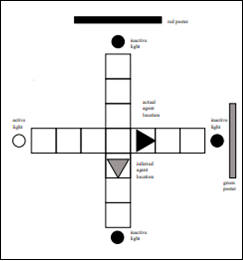
\includegraphics[width=0.5\textwidth]{figures/methods_size/plus_maze.png}
    \caption{The plus maze environment the model is learning, from \cite{foxandprescott2010A}}
    \label{fig:plus_maze}
\end{figure}

From how the CA3 sub-field is created, it provides two main options for increasing it's default size:
changing the environment the model learns and increasing the number of biases in the model.
Changing the environment would be impractical as multiple new environments that have different sizes would need to be created to fully explore how the time to learn changes as the CA3 sub-field increases in size.
On the other hand, increasing the number of biases in the model is trivial, and can be used to provide a comparison of how the time to learn is affected by multiple size changes to the CA3 sub-field.


% This makes the only options for increasing the size of the CA3 changing the environment the model learns, or increasing the number of bias nodes in the CA3 sub-field.
% Changing the environment would be impractical as a new environment of different size is needed to show how the model scales. 
% In addition, from how the CA3 is currently created, it is non-trivial to create a large environment for the model to learn.
%  \wording
% On the other hand, it can be considered trivial to add bias nodes to the creation of the CA3 sub-field.
% This allows for the model to be horizontally scaled quickly and easily, with the option to change the amount of extra nodes added.

We expect to see that the more nodes we add to the CA3, the time taken to train increases at a constant rate.
On the CPU version, we would expect to see a steep increase in time taken, whereas the GPU version would be a more gradual increase.


A problem that occurs when increasing the size of the CA3 sub-field is the increase in memory usage.
This is because Tensorflow converts from NumPy floating point arrays and Python floating point numbers to a 64 bit floating point tensor of the same size.
This is not suitable for GPU processing.
This is because GPU's have the best efficiency when working on 32 bit floating point numbers.
Whilst this change does reduce the overall precision of the model, for the purposes of this experiment, it can be considered to have a negligible effect on the results.

\subsection{Results from increasing the size of the CA3 sub-field}
% Plot this data as a graph? Might look better and would break the monotone document with some colour
As the number of neurons increases, the amount of calculations increases. 
Naturally this increases the amount of time the system needs to learn.
As can be seen from \tableref{tab:results_table_size}, increasing the size of the CA3 subfield also increases the time required to train the system.
\begin{table}[ht]
    \centering
        \begin{tabular}{|c|c|c|}
            \hline
            Number of Nodes in CA3 & Time Taken CPU (s) & Time Taken GPU (s) \\\hline
            86      & 83.3           & 335.6          \\ \hline
            1086    & 770.3          & 441.3          \\ \hline
            2086    & 2437.2         & 625.7          \\ \hline
            3086    & 4653.8         & 896.9          \\ \hline
            4086    & 7391.2         & 1231.5         \\ \hline
            5086    & 10337.4        & 1642.0         \\ \hline
            6086    & 14137.6        & 2154.4         \\ \hline
            7086    & 19531.4        & 2739.1         \\ \hline
            8086    & 24685.6        & 3423.7         \\ \hline
            9086    & 27058.8        & 4155.0         \\ \hline
        \end{tabular}
    \caption{
        Time taken to run the training process for different sizes of an artificially inflated CA3 using the model variations from test 0 and test 17.\footnotemark
    }
    \label{tab:results_table_size}
\end{table}



As we linearly increase the number of nodes from 3086, it requires approximately 3600 seconds (1 hour) more time.
In contrast, using the parallelised Tensorflow version, we only require approximately 420 seconds (7 minutes) more time for increased nodes.
This is a speed up of roughly 10 times for extra nodes.
These times were recorded on the implementations of Test ID 0 for the CPU version and Test ID 17 implementation for the GPU version.


\footnotetext{See \footref{foot:system} for system details.}
\section{Optimisation of data type casting}
Relating to the data type optimisation, data type casting is an expensive operation.
This is due to the need to reassign memory to match the new data type.
This does not affect the conversion from NumPy arrays to Tensorflow tensors as they are initialised as 32 bit floats.
However the model uses a comparison of probability against random values to create a new hidden state representation after fusing the probabilities from the different inputs.
This creates a boolean tensor.
NumPy is able to utilise Python's weak typing to use a boolean tensor as a numerical representation, but Tensorflow uses strong typing.
This causes us to need to cast the boolean values to float values.
As this is happening multiple times in every step of the learning process, it provides a candidate for optimisation.

\subsection{Results from optimising the casting operation}
One method for optimising the casting operation is to use the \mono{tf.where} function.
This creates a tensor of two values using a conditional statement to determine which value to use.
This is useful as the \mono{tf.where} function performs the same operation as casting.
Using the Timeit module, we can test whether this operation is faster than casting.

\begin{table}[ht]
    \centering
    \begin{tabular}{|c|c|c|}
        \hline
        Number of Nodes & tf.cast & tf.where \\ \hline
        10              & 62.073  & 43.839   \\ \hline
        100             & 62.091  & 43.934   \\ \hline
        1000            & 62.208  & 44.035   \\ \hline
        10000           & 61.614  & 44.288   \\ \hline
    \end{tabular}
    \caption{Timing 100000 invocations of each function over different numbers of nodes. The times reported are cumulative of all 100000 invocations.
    % Test to see whether \mono{tf.where} is an optimisation over casting for different numbers of units for 100000 invocations.
    }
    \label{tab:cast_v_where}
\end{table}


From \tableref{tab:cast_v_where}, it can be seen that there is a noticeable speed up by using \mono{tf.where} across different numbers of nodes.
This implies that implementing this optimisation into the model will reduce the overall time taken to learn.
After implementing the optimisation into the model, we get an average runtime of 332.2 seconds.
This is a minor improvement over the implementation of test ID 17, however it is an improvement thus we will be using this optimisation in future experiments. 
\section{Optimisation of the error function}
We can use line profiling to identify other areas of optimisation.
An example of this is the error function, which takes up ~20\% of the execution time. 
This makes it suitable candidate for optimisation.
Looking at the code in \coderef{code:errorfunc}, lines 2, 3, and 5 are element-wise operations, meaning that the parallelisation of these operations are simple, as Tensorflow tensors can already handle them.
The interesting line in this code is line 4.
This is because the Python keyword \mono{sum} performs a serial operation, which is inherently slow, and has no direct counterpart in Tensorflow.
However, there is a similar function, \mono{tf.reduce\_sum} which exhibits the same behaviour in a parallel manner.
\begin{minipage}{\linewidth}
\begin{lstlisting}[caption=Error function split into each operation, label=code:errorfunc,language=python]
def err(probabilities, hidden_state):
    difference = probabilities-hidden_state
    squared_difference = difference ** 2
    sum_difference = sum(squared_difference)
    error = sum_difference / hidden_state.shape[0]
    return error
\end{lstlisting}
\end{minipage}

\subsection{Results from optimising the error function}
\label{subsec:res_sum}


As seen in \tableref{tab:sum_v_reduce}, \mono{tf.reduce\_sum} maintains a relatively constant time regardless of the number of nodes used. 
This indicates that the optimisation is useful for reducing the overall learn time of the model, when comparing against a pure CPU implementation.

\begin{table}[ht]
    \centering
    \begin{tabular}{|c|c|c|}
        \hline
        Number of Nodes & sum (s)   & tf.reduce\_sum (s)\\ \hline
        10              & 0.183     & 0.018             \\ \hline
        100             & 1.496     & 0.011             \\ \hline
        1000            & 14.652    & 0.010             \\ \hline
        10000           & 144.899   & 0.011             \\ \hline
    \end{tabular}
    \caption{ Timing 100 invocations of the named functions across different numbers of nodes. The times reported are cumulative of the 100 invocations. }
    \label{tab:sum_v_reduce}
\end{table}

Implementing this optimisation into the model using 86 nodes in the CA3, we obtain an average runtime of 331.1 seconds. 
This is another minor improvement alongside the casting optimisation above, indicating that there is still a bottleneck in the code.
However, when the model is trained to learn a larger area, with more nodes, this optimisation will be beneficial.

% 336.378 seconds with tf.reduce sum

% \noteGeneral{This needs re-writing, checking on the 20th August shows there may be improvements from it, but not enough time to implement them and get results.}
% \textsc{
% As mentioned above, the optimisation of the error function looks to be very useful.
% After integrating the new error function into the system, we run 5 invocations of it using test ID 17 as a base.
% This gave an average runtime of the learning process of \noteGeneral{800} seconds, compared to the base time being 350 seconds.
% This is the opposite of what was expected, and as such this optimisation idea will not be used going forward.
% As we are using version control software to manage each revision of the model, we can easily rollback the model to a base state.\noteGeneral{Is this sentence necessary, I think it is, however feels like fluff.}}


\section{Profiling Results}
% Should include figures for initial implementation and the final implementation(Test id 15)
\subsection{Number of calls}
From \figureref{fig:ncc} we can see that the most called function, a lambda in the SURFExtractor module is part of the setup process, meaning the relevant functions are \mono{boltzmannProbs} in the rbm module, the \mono{fuse} function from the cffun module and the \mono{err} function in the learn weights module.


\begin{figure}
    \centering
    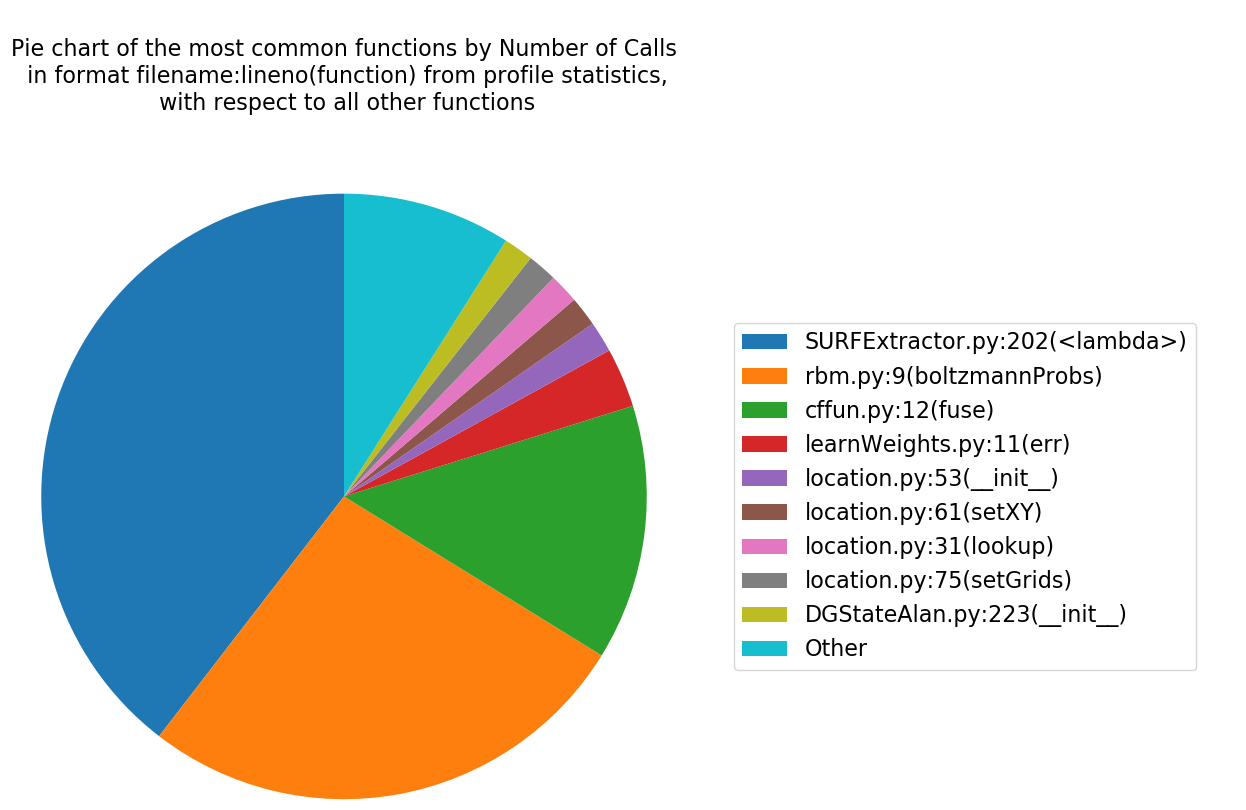
\includegraphics[width=0.7\textwidth]{figures/res_profiling/number_calls_cpu_crop.png}
    \caption{Number of calls for the CPU implementation of the model.}
    \label{fig:ncc}
\end{figure}

\begin{figure}
    \centering
    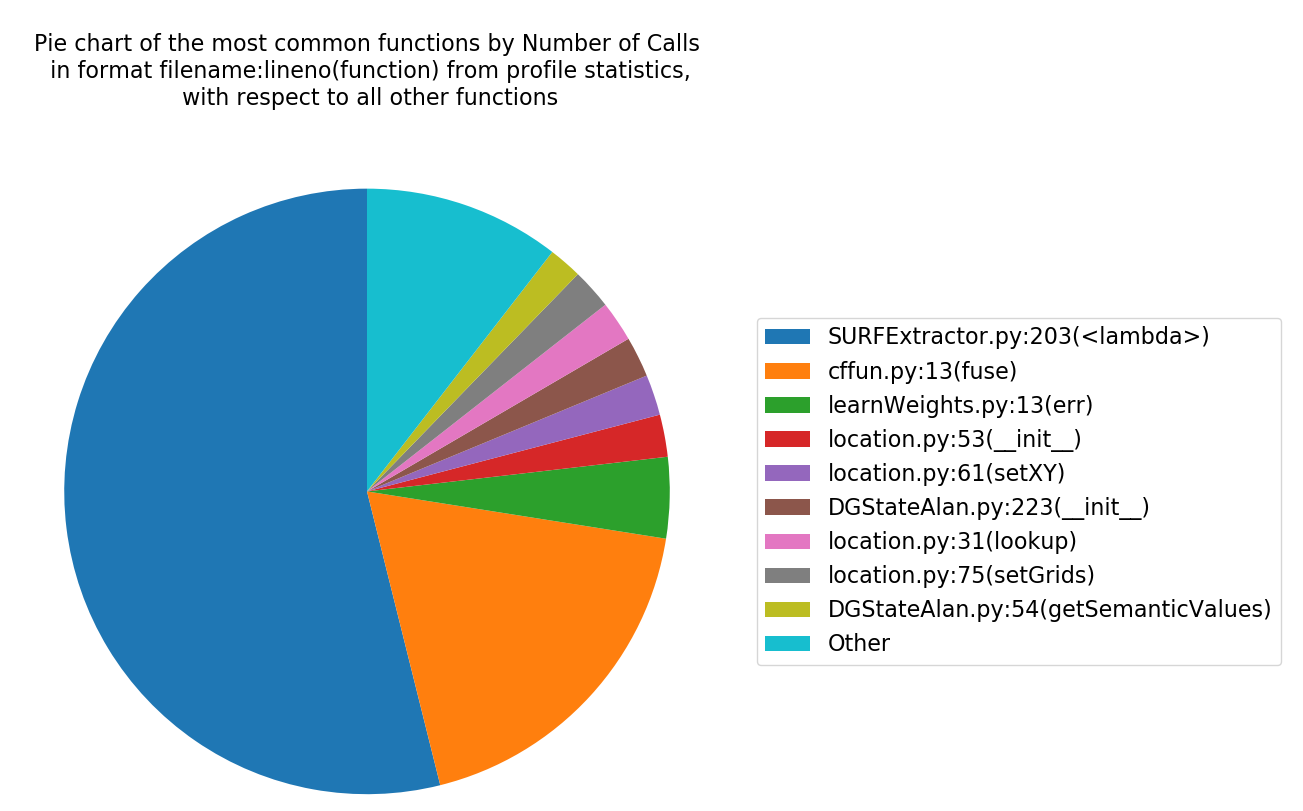
\includegraphics[width=0.7\textwidth]{figures/res_profiling/number_calls_gpu_crop.png}
    \caption{Number of calls for the GPU implementation of the model.}
    \label{fig:ncg}
\end{figure}

In contrast, profiling the Tensorflow version (\figureref{fig:ncg}) shows the lambda function from SURFExtractor taking a larger proportion of the total number of calls.
This is likely due to the usage of the \mono{tf.function} decorator optimisation.
The decorator converts the function into an optimised Tensorflow data call graph, which is loaded into the memory of the GPU at runtime.



Tensorflow processes the calls to the function such that the profiler only records the first time each call to \mono{boltzmannProbs} is hit, as opposed to everytime.
The \mono{cffun\#fuse} function has approximately the same amount of calls, and can probably be reduced by applying the \mono{tf.function} decorator.
Finally the \mono{learnWeights\#err} function has a constant number of calls across both implementations as it is not affected by the randomness of the model.


\subsection{Total time}

The more interesting profiling results come from the total time spent executing the function, excluding calls to other functions.
Initially the main functions that take the most time are the \mono{learn} function of the \mono{learnWeights} module, the \mono{boltzmannProbs} function of the \mono{rbm} module and the \mono{fuse} function of \mono{cffun} module as seen in \figureref{fig:ttc}.

After applying the parallel refactoring, the \mono{learnWeights\#learn} function takes a larger proportion of the overall time taken, as seen in \figureref{fig:ttg}.
The \mono{cffun\#fuse} function also has an increase in the proportion of time taken.
However, given that the overall time taken increases with a small amount of nodes, it indicates that there may be an underlying algorithmic problem which causes this behaviour.

\picturesque{figures/res_profiling/tot_time_cpu_crop.png}{Total time for function calls for the CPU implementation of the model.}{fig:ttc}

\picturesque{figures/res_profiling/tot_time_gpu_crop.png}{Total time for function calls for the GPU implementation of the model.}{fig:ttg}


In addition, the \mono{boltzmannProbs} function appears to have a large reduction in time taken.
However this is likely due to the \mono{tf.function} decorator function mapping the original function to a data call graph that runs purely on the GPU, which the Python profiler does not have access to.
This can be seen when using the line profiler on the \mono{boltzmannProbs} function.

%insert listing or similar thing depicting the output of line profiler, with full excerpt in an appendix.
\coderef{profiling:line_boltzmann} shows the results of profiling the \mono{boltzmannProbs} function line by line. 
It can be seen that the main bottleneck is the multiplication of the inputs and weights, taking approximately 60\% of the overall time.
This is likely due to the asynchronous nature of matrix multiplication, which is applied across a given dimension of the inputs. 


\begin{minipage}{\linewidth}
\begin{lstlisting}[caption=Line by line profiling of the rbm\#boltzmannProbs function in eager execution mode, label=profiling:line_boltzmann]
Total time: 237.186 s
Function: boltzmannProbs at line 9

Line #      Hits         Time  Per Hit   % Time  Line Contents
==============================================================
     9                                           @profile
    10                                           #@tf.function
    11                                           def boltzmannProbs(W, x, axis=0):      # RETURNS THE PROBABILITY OF A NODE BEING ON
    12    252240  143312866.0    568.2     60.4      mult = tf.tensordot(W, x, axis)
    13    252240   12193753.0     48.3      5.1      squeezed = tf.squeeze(mult)
    14    252240    6917896.0     27.4      2.9      E_on  = -squeezed       #penalty is the negative of the reward (just to make it look like energy
    15    252240   20604441.0     81.7      8.7      E_off = 0.0*E_on
    16    252240   13057317.0     51.8      5.5      Q_on = tf.math.exp(-E_on)       #as energy is negated, we have e^(reward)
    17    252240   12601996.0     50.0      5.3      Q_off = tf.math.exp(-E_off)
    18    252240   28258157.0    112.0     11.9      P_on = Q_on / (Q_on + Q_off)
    19    252240     239234.0      0.9      0.1      return P_on
\end{lstlisting}
\end{minipage}




\section{Verification of model accuracy}
The results outlined above only consider the learning process.
However for our optimisations to be considered successful, we need to compare the accuracy of the initial serial implementation of the model with the current parallelised implementation.


\begin{table}[h]
    \centering
    \begin{tabular}{|c|c|c|c|}
        \hline
        Version & Learned Weights   & Handset Weights   & Random Weights    \\\hline
        CPU     & 63.70\%           & 62.33\%           & 19.37\%           \\\hline
        GPU     & 41.93\%           & 67.27\%           & 19.37\%           \\\hline
    \end{tabular}
    \caption{
        Table comparing the accuracy of the model with respect to a 3000 step walk in the plus maze for each type of learning method, using handset weights, learned weights and random weights.
    }
    \label{tab:res_Metrics}
\end{table}

\tableref{tab:res_Metrics} shows the accuracy of the model for both the original CPU implementation and our parallelised implementation.
We consider 3 types of weights, weights learned from our learning process, handset weights of the model and random initialisation of weights.
For the random initialisation of weights there is no change in accuracy. 
This is due to the seed for initialising the weights being the same across both models.

With the handset weights, our implementation shows an overall increase of 5\% in Accuracy.
This suggests that the parallelised model obtains a more accurate picture of it's environment when given a good starting weight value for each area of the model.
However there is a loss of 20\% accuracy when using learned weights from the learning process.
This implies that there is an error in our learning process that affects the overall accuracy.

The next step from this is to add unit tests to both the learning and the evaluation process.
These tests would be targeted to capture the behaviour which causes the learned accuracy to be reduced.
This would allow the problem to be investigated and fixed, and would improve the accuracy to being approximately the same as the initial, CPU version.


% Conclusions
\chapter{Discussions and Conclusions}
{
% Our work was effective and does reduce time to learn when CA3 is large.
% However current environment does not reflect this as it is too small.
% This suggests that a new toy environment should be created and used as a comparison.
% This is due to artificial inflation of the RBM, and not actual increase in size.
}
{
Our results indicate that we have achieved our goal, especially when the size of the CA3 is large, which makes the model more suitable for real world use. 
However the environment is relatively small, and the inflation of the CA3 sub-field can be considered artificial.
This means that there may be a small performance improvement for a larger environment.
This can be checked by using the current parallel implementation in a new environment which covers a larger and more complex environment in future work.
}

{
% We assume that tensorflow is the best for the parallelisation
% However there are multiple libraries that achieve the same objective.
% Further work can be done to optimise the process by changing which parallelisation library is used as tensorflow does contain a large amount of overhead.
}

{
Next, we assumed that Tensorflow was the best option for parallelisation.
This is because of its popularity and prominence as a machine learning library.
However, as we outline in \sectionref{subsec:highlevellibs}, there are many libraries for Python which handle parallelisation and scaling.
As such we may be able to obtain better results from a different library.
This is because Tensorflow has initialisation overhead on first call, which can slow down the learning process, whereas other libraries will have different points of initialisation overhead, or does not load unnecessary modules, e.g. Keras. 
}

{
% Our initial profiling showed that the learning process was slow.
% This became the focus of our optimisations for time.
% However we do not verify that the optimisations implemented provide similar accuracy to initial results.
% Whilst this verification is not an issue for this project, if the model is to be deployed the verification would need to be heavily scrutenised as part of the deployment process.
}

{
Profiling the code showed that the learning process was slow.
This made it the best segment to optimise.
However our results indicate that the optimisation is only effective at scale.
We can assume that the problem lies within the matrix multiplication of each type of sensory/weight data in the model, (data from sensors, odometry data, recurrent neurons in the CA3 and the biases) when looking at the current environment.
This suggests that further work into optimising this multiplication will heavily reduce the overall time to learn, given that particular multiplication occurs ~250,000 times.

Furthermore, our secondary metric of model accuracy shows that our refactoring of the model is less than satisfactory.
This is because of the dramatic loss of accuracy of the learned weights.
However, our refactored model still performs twice as well as randomly selecting weights.
The model is also influenced by randomness, which may have played a part in how well the model learns, considering only 10 epochs are used during the training process.
This indicates that further work needs to be done to understand how the model reacts to randomness, and how that affects the overall accuracy of the model.

}

{
% Consider randomness and how that affects our results. (This might be better in the reflection)

Whilst we attempted to account for as many variables as possible within the optimisation process, the overall randomness of the model causes variations within results to occur.
An example of this is the model randomly choosing to account for observations and recurrent values in the  contrastive divergence learning.
This can be managed by setting a seed, however the asynchronous nature of parallel computing means that different threads can retrieve the next number in the random number generation in a different order with successive invocations.
Thus we chose to allow for the randomness to affect the learning process to provide us with a set of results that can be expected in a real world environment. 
}

% \noteComment{In Conclusion....}

{
In conclusion, our results show that our current optimisations only have an effect on the model at scale.
This is useful as real world environments are larger than the plus maze environment the model currently learns.
Finally, we have laid the foundations for future work to build upon our current refactoring of the model to Tensorflow using unit tests.

}



% end of thesis body
% --------------------------

% Print out the references
\pagebreak
\phantomsection
\addcontentsline{toc}{chapter}{References}
\printReferences


% Acknowledgements


\renewcommand{\chaptername}{Appendix} % To change title from chapter to Appendix
\appendix
\chapter{Additional assessment information}


We have written this report in the form of a scientific paper as we plan to publish it. 
However the MSc Research Project assessment criteria requires additional information that is not usually included in publications.
As such, we include this information below.
%  This report has been written in the format of a scientific paper as we plan to publish it. The MSc assessment criteria requires some additional information not usually included in publications, so we include this below.

\section{Aims and objectives}
The aim of the project is to use Tensorflow to parallelise a model of the hippocampus to make it more suitable for real-time/real world use. To do this we will need to complete the following objectives:
\begin{itemize}
    \item Write unit tests to understand current system behaviour
    \item Ensure the initial implementation passes unit tests.
    \item Write Tensorflow-based Python code that emulates current system behaviour.
    \item Verify our Tensorflow code works as expected using the unit tests.
    \item Time the system using different combinations of the original code and parallel code,
    \item Profile the final system and compare it to our original profiling results.
\end{itemize}

% This section is probably not necessary however I am putting this down as part of ticking the boxes of the brief.
% \subsection{Hypothesis}
% The hypothesis of this project is that moving the model to train on the GPU will cause the model to run faster at scale. 
\section{Tools and Toolsets}
% This covers things not in the lit review, going by kai's things like IDE, automation scripts etc.
As a software engineering project, we will need to use tools outside those covered above to manage the development of the model.

\subsection{Development Environment}
% Ubuntu 18.04
% What is Jetbrains Intellij Idea, why was it useful (i.e. integration with python, git shell, ?csv files?
% Python 3.6 and libraries w/ versions.(List)
% Automation scripts with shell. (simulate how system would work on robot?)
The model is developed on Linux, as it would be a similar operating environment that would be used in the real world.
We use Jetbrains Pycharm as our development environment as it provides quality of life features such as code completion and inspection. 
It also has integration with Git which makes it easier to see which files have been modified.
This helps in managing which functions have been integrated into the system as a whole.
It also allows for the management of virtual Python environments, which separate Python libraries to reduce confusion on which libraries to use. 
Below is a list of libraries that need to be installed into the environment in order to obtain a minimum working environment.

\begin{itemize}
    \item Pip version: 20.1.1
    \item NumPy version: 1.18.4
    \item Matplotlib version: 3.2.1
    \item Pyflann3 version: 1.8.4.1
    \item Opencv-contrib-python-nonfree version: 4.1.1.1
    \item Tensorflow version: 2.2.0
\end{itemize}

\subsection{Git and Github}
% What is Git
% Why did we use it.
Git is a version control tool.
It records changes to files in a tree based manner.
This is useful for our project as it provides a method to return to a previous model state quickly and easily.
This allows for different paths that the model can be developed in to be explored, which makes overall development faster.
In addition, it also acts as a backup mechanism, by regularly pushing updates to repository sites like Github, as it allows the model to be restored at any time in the event of hard drive failure or loss of data.
% \footnote{All results can be found at https://github.com/a\-yakkus/hclearn/wiki/results2020}
% TODO convert to link. This is the table in my research journal.


\subsection{Latex and Overleaf}
% What is Latex
% Why did we use it.
Latex is a typesetting system.
This allows it to have a singular source, but provide different document layouts.
This makes it easier to convert the report to different formats for publication.
There are multiple environments for processing latex documents, such as Overleaf, TexLive and MikTex.
We chose Overleaf as it is an online environment, which suggests that there is some form of redundancy measures in place.
This is useful as it means that if a local drive was to fail, the report would not be lost.
In addition, an online environment allows for easy collaboration with others. This makes it easier to work with my supervisor and proofreaders, as discussions on minor changes can be made quickly and easily.
Another reason for choosing Overleaf instead of Texlive and MikTex is that it is a managed system.
This means that extra packages, such as table/figure rendering and placement are instantly available.
Whilst these packages can be installed into a TexLive or MikTex environment, it would slow down the creation of the report.
Finally, in order to convert latex source to a suitable document for submission, it is customary to compile the same source code multiple times to fix intradocument referencing. 
This can be done in the other environments, however Overleaf provides a partially parsed log when compilation fails, which makes it easier to identify the problem and fix it as opposed to the other environments which would require identifying the problem from the logs. % Which has already been done enough in this project from python + tensorflow in order to get a working prototype to push to git/time. 



\section{Project Management}
When developing software, there are multiple methodologies that can be applied, such as Agile and Waterfall.
However our project revolves around refactoring an initial software package.
This makes the Waterfall methodology unsuitable for the project, as the requirements are subject to change after each optimisation after refactoring.
Agile practices, on the other hand are more suitable for our project.
This is because the intermediary goals, such as which function to optimise next changes after each build of the system.
This allows us to move fluidly through the development of parallel versions of the function, with no strict oversight on what should be done next.

As test driven development uses short software cycles to develop functions, it works well with an Agile approach.
Furthermore, test driven development is suitable for refactoring as it allows us to manage deterministic behaviour easily.
This means that if a function does not pass the tests, then it enables the developer to revisit the function and work out where the error that causes the test to fail occurs.
Test driven development has been useful for this project in ensuring that behaviour is correct of our refactored functions.
\subsubsection{Risk Matrix}
% TODO table of risks
% Ideas:
% Computer breaks (CPU/GPU)
% Data loss (i.e. hard drive failure)
% Deviation from plan
% Poor use of Version Control
% 
When doing a software engineering project, there are risks that can occur during the project. We display these risks in \tableref{tab:risks}.

\begin{table}[ht]
    \centering
    \resizebox{\linewidth}{!}{
        \begin{tabular}{|p{2.5cm}|p{1.5cm}|p{1.5cm}|p{2cm}|p{5cm}|}
            \hline
            Risk & Severity Level & Impact & Likelihood & Mitigation  \\ \hline
            Hardware failure & 4 & 4 & 1 & Replace failed components of the machine with the same component \\ \hline
            Data Loss & 3 & 3 & 2 & Regularly back up data to multiple external sources\\ \hline
            Deviation from main optimisation points & 1 & 4 & 3 & Focus mainly on the big optimisations, and return to smaller optimisations at a future point in time. \\ \hline
        \end{tabular}
    }
    \caption{Risk matrix for project.}
    \label{tab:risks}
    
\end{table}



% PLan for reflective analysis, paragraph for each, maybe 2 for last point, aim for ~1pg
% What went well? (Unit testing, integration testing of independent functions)
% What did not go well? (Integration of dependent functions)
% Compare to bachelors (did what I learn carry forward?, how do the projects differ?)
% What could I have done better (Verification that accuracy remains similar +-5%, more rigourous testing, learning more about tensorflow 1 and 2 near the start of the project, followed test driven development rigour better)
\section{Reflection}
This project has been an enjoyable process for me.
It has allowed me to expand my knowledge of different machine learning models and techniques.
I usually use an iterative Waterfall approach to software development, using unit tests has been a welcome change of pace.
It made the overall development of the project a lot smoother as it helped me understand the purpose of each function used in the learning process, and how they interact between each other.

The overall process of the development of the parallel version was smooth. 
This was due to the unit tests making it easier to see where problems were and how they may affect future model development over different iterations.
By using unit tests in this project, I have found that there are more benefits to using unit tests than not using them, which I will be using in future projects.

When considering what did not go well, it was mainly the integration of each function into the overall system.
This is because of the difference between Tensorflow and NumPy with different implementations of functions, such as the dot product.
This caused a variety of solutions to be created to manage this, however they all had some variation that means they may not have been optimal.
Another problem from the project is that the speed up seen in experimental results is not as expected, with approximately 2x speed up occurring at 1000+ neurons, and approximately 7x speed up at 3000+ neurons, whereas we were expecting to see around a 100x speed up with larger network sizes.

In comparison to my bachelors project, I feel this project has been more successful. This was likely due to the extra time that could be dedicated to the project, without other assignments to worry about.
Another reason for this project being more successful is that I was able to take lessons learned from my bachelors project, such as involving my supervisor more and using more resources available to me.

If I was to redo this project, I would focus more on understanding different parallel frameworks before beginning development, and how different versions of these libraries affect their performance.
Another thing that I would redo is to be more rigorous in following test driven development, as I have developed a parallel function before the tests.
This had a negligible effect on the development of the software, but does encourage poor habits when developing code.

%  \chapter{Data}
%  % \begin{minipage}{\linewidth}
\subsubsection{LearnWeights\#learn}
\begin{lstlisting}[xrightmargin=0.05\linewidth,caption=Line by line profiling of the learnWeights\#learn function (boltzmann probs as an eager function), label=profiling:line_learn]
Total time: 529.294 s
File: /home/yakkus/github/jack-fork/hclearn/workspace/src/main/learnWeights.py
Function: learn at line 21

Line #      Hits         Time  Per Hit   % Time  Line Contents
==============================================================
    21                                           @profile
    22                                           def learn(path, dictSenses, dictGrids, N_mazeSize, ecs_gnd, dgs_gnd, ca3s_gnd, b_learnIdeal=True, b_learnTrained=False, b_learnDGWeights=True, learningRate=0.01):
    23         1          4.0      4.0      0.0      dghelper=None
    24                                               #Learn DG weights when you have visual input
    25         1          3.0      3.0      0.0      if b_learnDGWeights:
    26                                                   #Extract data from dictionary of senses to train on 
    27         1         14.0     14.0      0.0          allSURFS = [ sense.surfs for sense in dictSenses.values() ]
    28                                                   #print allSURFS
    29                                                   #print len(allSURFS)
    30                                           
    31                                                   #Select a selection?
    32         1          3.0      3.0      0.0          percent = 100
    33         1          5.0      5.0      0.0          numOfImages = int(len(allSURFS)*(percent/float(100)))
    34         1          4.0      4.0      0.0          allIndices = range(0,len(allSURFS))
    35                                                   #print(allIndices)#debug as part of python3 update process
    36         1         19.0     19.0      0.0          np.random.shuffle(list(allIndices))# convert to list as range does not support getItem
    37         1          5.0      5.0      0.0          randomIndices = allIndices[0:numOfImages]
    38         1         10.0     10.0      0.0          randomSURFs = [ allSURFS[ind] for ind in randomIndices ] 
    39                                           
    40                                                   #Train weights
    41         1          3.0      3.0      0.0          X=7
    42         1          3.0      3.0      0.0          N=45
    43         1          3.0      3.0      0.0          presentationOfData = 30
    44         1          3.0      3.0      0.0          learningrate = 0.05
    45         1     931414.0 931414.0      0.2          dghelper = DGStateAlan.train_weights(randomSURFs, X, N, presentationOfData, learningrate)
    46                                           
    47                                               #Learn ideal weights (with perfect look ahead training)
    48         1          4.0      4.0      0.0      if b_learnIdeal: #latest :  lots of odom noise    
    49                                                   #print ("TRAINING IDEAL WEIGHTS...")
    50         1    5588541.0 5588541.0      1.1          (ecs_nsy, dgs_nsy, ca3s_nsy) = path.getNoiseyGPSFirings(dictSenses, dictGrids, N_mazeSize, dghelper)  #ideal percepts for path, for trainign and for inference
    51                                           
    52         1    7426839.0 7426839.0      1.4          senses = ecs2vd_so(ecs_nsy,dictGrids, dghelper) 
    53                                           
    54                                                   #Use test2.py for learning, use this for generating ground truth path to learn with test2.py
    55         1     310995.0 310995.0      0.1          odom   = ecs2vd_oo(ecs_nsy,dictGrids) 
    56         1      80641.0  80641.0      0.0          hids   = ca3s2v(ca3s_gnd) ##NB this is the ground truth, no noise
    57                                           
    58         1        830.0    830.0      0.0          WB = trainPriorBias(hids)
    59                                           
    60         1   19120224.0 19120224.0      3.6          WR = trainW(lag(hids,1), hids, WB, N_epochs=1, alpha=0.01)
    61         1   18793573.0 18793573.0      3.6          WS = trainW(senses,      hids, WB, N_epochs=1, alpha=0.01)
    62         1   17906180.0 17906180.0      3.4          WO = trainW(odom,        hids, WB, N_epochs=1, alpha=0.01)
    63                                           
    64         1       1552.0   1552.0      0.0          np.save(pathing+"WR",WR)
    65         1       1768.0   1768.0      0.0          np.save(pathing+"WS",WS)
    66         1       1016.0   1016.0      0.0          np.save(pathing+"WB",WB)
    67         1       1405.0   1405.0      0.0          np.save(pathing+"WO",WO)
    68                                           
    69         1       3423.0   3423.0      0.0          np.save(pathing+"hids",hids)
    70         1       1810.0   1810.0      0.0          np.save(pathing+"odom",odom)
    71                                           
    72         1      42292.0  42292.0      0.0          np.save(pathing+"senses",senses)
    73                                                
    74                                                   #print ("DONE TRAINING")
    75                                           
    76         1         11.0     11.0      0.0      if b_learnTrained:
    77                                                   #print ("TRAINING TRAINED WEIGHTS...")
    78                                           
    79                                                   #foo = np.random.random()
    80                                           
    81         1       3884.0   3884.0      0.0          WR = np.load(pathing+'WR.npy')
    82         1       3306.0   3306.0      0.0          WO = np.load(pathing+'WO.npy')
    83         1       2342.0   2342.0      0.0          WS = np.load(pathing+'WS.npy')
    84         1       1102.0   1102.0      0.0          WB = np.load(pathing+'WB.npy')
    85         1          6.0      6.0      0.0          WB = WB[...,tf.newaxis]
    86                                                   #WB=WB.reshape((,1))
    87                                                   #No longer need the above lines as they are a hack and the wrong size
    88                                           
    89                                                   ##these are all to be learned, so overwrite them with rands
    90         1        237.0    237.0      0.0          WR = tf.convert_to_tensor(1-2*np.random.random(WR.shape), dtype=tf.float32) #Weights recurrent
    91         1         61.0     61.0      0.0          WB = tf.convert_to_tensor(1-2*np.random.random(WB.shape), dtype=tf.float32) #Weights bias
    92         1         88.0     88.0      0.0          WO = tf.convert_to_tensor(1-2*np.random.random(WO.shape), dtype=tf.float32) #Odom sensors
    93         1       1011.0   1011.0      0.0          WS = tf.convert_to_tensor(1-2*np.random.random(WS.shape), dtype=tf.float32) #Non-odom sensors - INCLUDING SURF - Need to include DG size within it
    94                                                   #ALAN Seems like by changing the ecs2vs_so to include the surf features this size has been now modified correctly?
    95                                                   #Above need resizing to include SURF weights
    96                                           
    97                                                   #hids_gnd=addBias(hids)    #NB each pop has a local bias, in addition to the global prior bias
    98         1       2339.0   2339.0      0.0          hids_gnd=addBias(np.load(pathing+'hids.npy'))    #NB each pop has a local bias, in addition to the global prior bias
    99                                                   #ALAN - Keep hids_gnd the same 
   100                                                   #odom=addBias(odom)
   101         1       1752.0   1752.0      0.0          odom=tf.convert_to_tensor(addBias(np.load(pathing+'odom.npy')), dtype=tf.float32)
   102                                                   #senses=addBias(senses)
   103         1      19276.0  19276.0      0.0          senses=tf.convert_to_tensor(addBias(np.load(pathing+'senses.npy')), dtype=tf.float32)
   104                                                   #ALAN - odom and senses are matrices with rows as time columns as what is observed at that time (light, whiskers, SURF, DGencodedSURF etc.)
   105                                           
   106         1       1608.0   1608.0      0.0          hidslag_gnd = tf.convert_to_tensor(lag(hids_gnd,1), dtype=tf.float32)
   107                                           
   108         1         47.0     47.0      0.0          T = odom.shape[0]
   109                                           
   110         1         66.0     66.0      0.0          b = tf.convert_to_tensor(np.array([1.0]), dtype=tf.float32)  #bias
   111         1          4.0      4.0      0.0          alpha = learningRate #0.01 ##0.0001 is stable, starting at perfects; 0.001 diverges.
   112         1         83.0     83.0      0.0          one_const = tf.convert_to_tensor([[1.]], dtype=tf.float32)
   113                                                   ### train with proper wake-sleep (no peeking at hid_t, though hid_{t-1} is OK )
   114                                                   
   115                                                   #FIXME: TURN BACK TO 1000 or so!
   116        11         38.0      3.5      0.0          for epoch in range(0,10):
   117        10         46.0      4.6      0.0                  err_epoch = 0  #accumulator
   118                                           
   119     30010     112829.0      3.8      0.0                  for t in range(0,T):
   120                                                               #print(epoch, t)
   121     30000     511954.0     17.1      0.1                      b_fakeSub = np.random.uniform()>0.5#tf.floor(2*tf.random.uniform(shape=()))  #learn on full data or on hist-indep subset?
   122                                           #                    print(b_fakeSub)
   123     30000    9168355.0    305.6      1.7                      hids_prev = hidslag_gnd[t,:]
   124     30000    8455224.0    281.8      1.6                      s = senses[t,:]
   125     30000    8390718.0    279.7      1.6                      o = odom[t,:]
   126                                           
   127                                                               #WAKE
   128                                           
   129     30000   29418596.0    980.6      5.6                      p_b  = boltzmannProbs(WB, one_const)
   130     30000   31658924.0   1055.3      6.0                      p_s  = boltzmannProbs(WS, s[...,tf.newaxis], 1)
   131     30000    1434544.0     47.8      0.3                      p = tf.identity(p_b)#.copy()
   132     30000    9986673.0    332.9      1.9                      p=fuse(p, p_s)
   133                                           
   134     30000     102497.0      3.4      0.0                      if not b_fakeSub:
   135     15030   15458254.0   1028.5      2.9                          p_o  = boltzmannProbs(WO,o[..., tf.newaxis], 1)
   136     15030   15264881.0   1015.6      2.9                          p_r  = boltzmannProbs(WR,hids_prev[..., tf.newaxis], 1)
   137     15030    4875694.0    324.4      0.9                          p=fuse(p, p_o)
   138     15030    4806321.0    319.8      0.9                          p=fuse(p, p_r)
   139                                           
   140     30000    7522842.0    250.8      1.4                      hids = tf.cast(p > tf.random.uniform(p.shape, dtype=tf.float32), dtype=tf.float32)#.astype('d')    #sample, T=1
   141     30000   14372749.0    479.1      2.7                      CS = cffun.outer(hids, s)
   142     30000   16153216.0    538.4      3.1                      CB = cffun.outer(hids, b)
   143     30000    4600414.0    153.3      0.9                      WS += alpha*CS
   144     30000    3982619.0    132.8      0.8                      WB += alpha*CB
   145     30000     111607.0      3.7      0.0                      if not b_fakeSub:
   146     15030    5906466.0    393.0      1.1                          CO = cffun.outer(hids, o)
   147     15030    5177314.0    344.5      1.0                          CR = cffun.outer(hids,hids_prev)
   148     15030    2192352.0    145.9      0.4                          WR += alpha*CR
   149     15030    1972498.0    131.2      0.4                          WO += alpha*CO
   150                                                               #SLEEP
   151                                           
   152                                                               #retain the hid sample from the wake step -- draw samples from obs, then hid again, CD style.
   153                                           
   154     30000     103955.0      3.5      0.0                      if not b_fakeSub:
   155     15030   18478766.0   1229.5      3.5                          po = boltzmannProbs(tf.transpose(WO), hids, 1)
   156     15030    3894712.0    259.1      0.7                          o = tf.cast(po > tf.random.uniform(po.shape, dtype=tf.float32), tf.float32)#.astype('d') #sleep sample (at temp=1)
   157                                                                   
   158                                           
   159     30000   36176475.0   1205.9      6.8                      ps = boltzmannProbs(tf.transpose(WS), hids, 1)
   160     30000    7707446.0    256.9      1.5                      s = tf.cast(ps > tf.random.uniform(ps.shape, dtype=tf.float32), tf.float32)#.astype('d')    #sleep sample (at temp=1)
   161                                           
   162     30000   28236783.0    941.2      5.3                      p_b  = boltzmannProbs(WB, one_const)
   163     30000   31887668.0   1062.9      6.0                      p_s  = boltzmannProbs(WS,s, 1)
   164     30000    1425667.0     47.5      0.3                      p = tf.identity(p_b)#.copy()
   165     30000    9992868.0    333.1      1.9                      p=fuse(p, p_s)
   166                                           
   167     30000     103945.0      3.5      0.0                      if not b_fakeSub:
   168     15030   15495164.0   1030.9      2.9                          p_o  = boltzmannProbs(WO, o, 1)
   169     15030   15334267.0   1020.2      2.9                          p_r  = boltzmannProbs(WR, hids_prev[..., tf.newaxis], 1)
   170     15030    4860711.0    323.4      0.9                          p=fuse(p, p_o)
   171     15030    4792349.0    318.9      0.9                          p=fuse(p, p_r)
   172                                           
   173                                                               #resample hids (needed to antii learn recs!)
   174     30000    7524468.0    250.8      1.4                      hids = tf.cast(p > tf.random.uniform(p.shape, dtype=tf.float32), tf.float32)#.astype('d')    #sample, T=1
   175     30000   14380460.0    479.3      2.7                      CS = cffun.outer(hids,s)
   176     30000   16193415.0    539.8      3.1                      CB = cffun.outer(hids,b)
   177     30000    4410385.0    147.0      0.8                      WS -= alpha*CS
   178     30000    3811475.0    127.0      0.7                      WB -= alpha*CB
   179                                           
   180     30000     112332.0      3.7      0.0                      if not b_fakeSub:
   181     15030    5822564.0    387.4      1.1                          CO = cffun.outer(hids,o)
   182     15030    5155719.0    343.0      1.0                          CR = cffun.outer(hids,hids_prev)
   183     15030    2086801.0    138.8      0.4                          WR -= alpha*CR
   184     15030    1870146.0    124.4      0.4                          WO -= alpha*CO
   185                                           
   186                                           
   187                                                               #TODO report error rate?
   188     30000   16043077.0    534.8      3.0                      e = err( hids, hids_gnd[t,:] )
   189     30000    1499515.0     50.0      0.3                      err_epoch += e
   190                              
   191                                           
   192                                           
   193                                                      # print('epoch:'+str(epoch)+' err:'+str(err_epoch))
   194                                           
   195         1       1488.0   1488.0      0.0          np.save(pathing+'tWR',WR)
   196         1       1677.0   1677.0      0.0          np.save(pathing+'tWS',WS)
   197         1       1299.0   1299.0      0.0          np.save(pathing+'tWB',WB)
   198         1       1263.0   1263.0      0.0          np.save(pathing+'tWO',WO)
   199                                               # 1 see if these give ok results
   200                                               # 2 try disbaling odom info again, and learning in its absence half the time 
   201                                           
   202         1          3.0      3.0      0.0      if b_learnDGWeights:
   203         1          3.0      3.0      0.0          return dghelper
\end{lstlisting}
% \end{minipage}

\end{document}
